\documentclass[11pt]{article}

\usepackage[margin=1in]{geometry}
\usepackage{amsmath,amssymb,amsthm,mathtools}
\usepackage{listings}
\usepackage{microtype}
\usepackage{graphicx}
\usepackage{float}
\usepackage{longtable}
\usepackage{tikz}
\usepackage[hidelinks]{hyperref}
\hypersetup{linktoc=all}
\setcounter{tocdepth}{2}
\makeatletter
\renewcommand{\l@subsection}{\@dottedtocline{2}{1.5em}{3.4em}}
\makeatother
\usetikzlibrary{arrows.meta,calc,positioning}

\newtheorem{theorem}{Theorem}
\newtheorem{lemma}[theorem]{Lemma}
\newtheorem{definition}[theorem]{Definition}

\title{CJR Core: Syntax, Semantics, and Separation Logic}
\author{Dan R. Ghica}
\date{\today}

\lstdefinestyle{coq}{
  basicstyle=\ttfamily\small,
  columns=fullflexible,
  keepspaces=true,
  showstringspaces=false,
  breaklines=true,
  frame=single,
  framerule=0.3pt,
  xleftmargin=0.4em,
  xrightmargin=0.4em,
  aboveskip=0.8em,
  belowskip=0.8em,
  literate={Σ}{{$\Sigma$}}1
           {↦ₛ}{{$\mapsto_s$}}2
           {↦ₒ}{{$\mapsto_o$}}2
           {λ}{{$\lambda$}}1
           {↦ₒ}{{$\mapsto_o$}}2
           {→}{{$\rightarrow$}}1
           {∀}{{$\forall$}}1
           {∃}{{$\exists$}}1
           {∗}{{$*$}}1
           {⌜}{{$\ulcorner$}}1
           {⌝}{{$\urcorner$}}1
           {≤}{{$\leq$}}1
           {∧}{{$\land$}}1
           {∨}{{$\lor$}}1
           {∈}{{$\in$}}1
           {⊢}{{$\vdash$}}1
           {≠}{{$\neq$}}1
           {∉}{{$\notin$}}1
           {∅}{{$\emptyset$}}1
}
\lstset{style=coq}

\newcommand{\cjr}{CJR}
\newcommand{\sem}[1]{[\![#1]\!]}
\newcommand{\step}{\longrightarrow}
\newcommand{\steps}{\longrightarrow^{*}}
\newcommand{\Stuck}{\mathsf{stuck}}
\newcommand{\WF}{\mathsf{wf}}
\newcommand{\dom}{\operatorname{dom}}
\newcommand{\lookup}[2]{#1(#2)}
\newcommand{\None}{\mathsf{None}}
\newcommand{\Some}{\mathsf{Some}}
\newcommand{\Unit}{\mathsf{()}}
\newcommand{\True}{\mathsf{true}}
\newcommand{\False}{\mathsf{false}}
\newcommand{\NULL}{\mathsf{null}}
\newcommand{\pts}{\mathrel{\mapsto}}
\newcommand{\ptss}{\mathrel{\mapsto_{s}}}
\newcommand{\ptsr}{\mathrel{\mapsto_{r}}}
\newcommand{\ptsb}{\mathrel{\mapsto_{b}}}
\newcommand{\ptso}{\mathrel{\mapsto_{o}}}
\newcommand{\sep}{\mathbin{*}}
\newcommand{\bigsep}{\mathop{\scalebox{1.4}{$\ast$}}}
\newcommand{\wand}{\mathbin{-\!\!*}}
\newcommand{\later}{\mathop{\triangleright}}
\newcommand{\Wpre}{\mathsf{wp}}
\newcommand{\GWpre}{\mathsf{gwp}}
\newcommand{\pure}[1]{\ulcorner #1 \urcorner}

\begin{document}
\maketitle

\begin{abstract}A tutorial on the CJR operational core, generic source layer, Iris contracts, and small extracted examples.\end{abstract}

\clearpage
\tableofcontents
\clearpage

\section{What this development is}

We take as our starting point a deliberately small core.
\cjr{} has a sequential untyped operational core and code pointers, so that a vtable can be written by hand.
An explicit rank-one generic source layer erases to that same core and extracts to native Cangjie generics.
Inheritance, interface bounds, higher-rank polymorphism, \texttt{enum}/\texttt{match}, and concurrency are outside this fragment.
Features of a larger source language that fall outside this cut are treated as sugar that must lower into the core at the same time and space cost.
What follows defines both the core and the explicit generic layer.
The function \texttt{erase} defines the latter's translation to the core.
There is no general Cangjie parser or lowering pass, garbage collector,
or byte-level layout model.

Safety, in this development, is not a type system.
The legacy grammar \texttt{ty} documents core representations. The separate
grammar \texttt{gty} records structured source types, including type variables
and named applications such as \texttt{Box<Pair<Int64, Bool>>}.
The generic checker validates names, scopes, and arities; it is not a complete
typing judgment. The operational semantics remains untyped.
A program is safe when a weakest-precondition proof exists; adequacy then says that, from the empty machine, execution does not get stuck.
Generic specifications quantify over Iris predicates describing element
representations. They prove uniform behavior of the supplied implementations;
they do not establish a general relational-parametricity theorem for all
well-typed Cangjie programs.

The Coq sources live under \texttt{theories/}.
The language is an Iris evaluation-context language~\cite{iris-ground-up,iris-essence}, so the frame rule and the bind rule are Iris's, rather than those of a separate Hoare calculus.
The overall shape follows HeapLang, the example language shipped with the Iris Coq development~\cite{iris-coq}.

\section{Tool structure and workflow}
\label{sec:tool-workflow}

The intended workflow starts with two related inputs.  The first is an
informal description of a data structure: its abstract contents, a concrete
representation, and the algorithms for its operations.  The second is a set
of properties that should validate the implementation.  These include the
main representation-correctness claims (for example, that an implementation
of list insertion produces the abstract list with the new element) and
equational client properties (for example, that adding an element and then
removing it restores the original list).  Such laws are separate obligations;
they do not follow merely from writing down the operations.

An engineer or an LLM can help translate the informal material into formal
definitions and theorem statements.  The formal development gives a
mathematical model of the abstract structure, a representation predicate
connecting that model to the CJR heap, executable CJR expression trees for
the operations, and specifications stated as weakest preconditions.  The
translation is a proposal that must be reviewed: informal text does not
become a theorem until its meaning has been made explicit in Rocq/Coq.
For generic programs, the executable definitions are \texttt{gexpr} trees
with explicit declaration references and type arguments. Their specifications
use the same Iris logic after erasure to \texttt{expr}; a declaration such as
\texttt{Box<T>.map<U>} is proved once against arbitrary input and output
representation predicates.

The proofs use Iris's separation logic over the small-step semantics of CJR.
The Iris weakest-precondition rules describe how each operation transforms
owned heap resources and establishes its postcondition.  The proved
implementation-correctness theorems connect the concrete representation to
the abstract model; algebraic laws can then be proved by composing those
verified operations.  Rocq/Coq's kernel checks the resulting proof terms.
In this repository the development is built with Coq 8.20.1 and Iris 4.4.0.
The language is called Gallina (two l's); Rocq is the prover, and Iris is the
program logic and library used for the heap reasoning.

Once the CJR definitions are available, \path{tools/extraction/rocq/emit_cj.v}
uses a custom Gallina printer to turn the selected CJR syntax trees into
Cangjie source files under \path{example/*/extracted/}.  This is not Rocq's
standard extraction mechanism, and it does not extract proof terms: it
serializes the program definitions.  A disciplined build runs
\texttt{make verify} to check proofs and assumptions, then \texttt{make cj}
to emit the programs.  Passing the proof check establishes the stated CJR
properties; by itself it does not prove that the printer's output preserves
the CJR semantics.
The original printing interface remains available for existing programs.
The generic path in \path{tools/extraction/rocq/generic_print.v} prints the
structured source directly, retaining type parameters and named layouts.
It does not try to reconstruct generic types from erased terms.

Finally, Cangjie unit tests compile and execute representative cases of the
generated code.  They are valuable sanity checks for the printer, compiler,
and runtime together, but they cover finitely many inputs and do not replace
the proofs.  The current project contains this formal semantics, Iris
proofs, custom printer, and runtime tests.  It does not yet implement an
automatic LLM front end that accepts arbitrary informal specifications.
The distinction between the proved CJR program and the tested emitted
Cangjie is important; Appendix~\ref{sec:limitations} records concrete risks
at that boundary.

\begin{figure}[H]
\centering
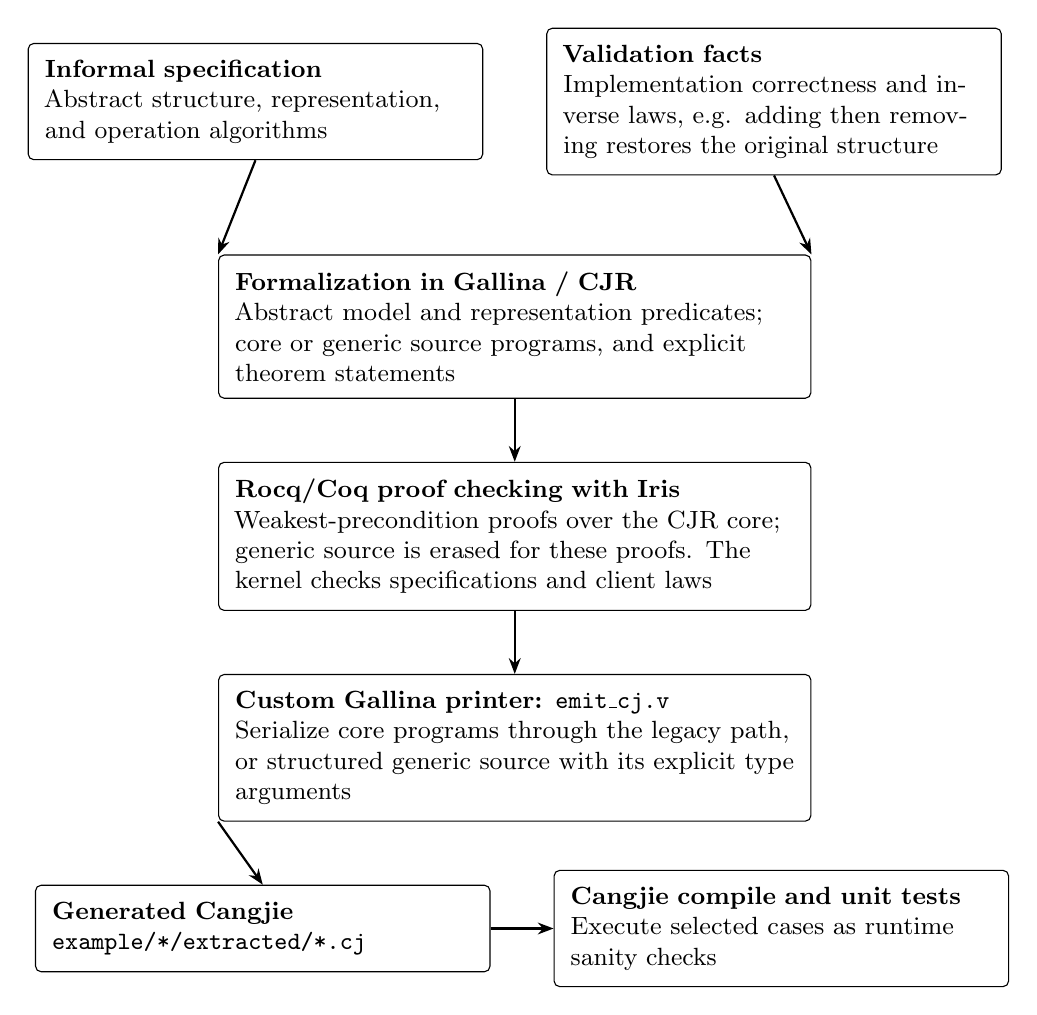
\begin{tikzpicture}[
  box/.style={draw, rounded corners=2pt, align=left, text width=5.35cm,
              inner sep=6pt, font=\small},
  process/.style={draw, rounded corners=2pt, align=left, text width=7.1cm,
                  inner sep=6pt, font=\small},
  arrow/.style={-{Stealth[length=2mm]}, thick}
]
\node[box] (informal) {\textbf{Informal specification}\\
  Abstract structure, representation, and operation algorithms};
\node[box, right=8mm of informal] (facts) {\textbf{Validation facts}\\
  Implementation correctness and inverse laws, e.g. adding then removing
  restores the original structure};
\node[process, below=11mm of $(informal.south)!0.5!(facts.south)$] (formal) {
  \textbf{Formalization in Gallina / CJR}\\
  Abstract model and representation predicates; core or generic source
  programs, and explicit theorem statements};
\node[process, below=8mm of formal] (proof) {
  \textbf{Rocq/Coq proof checking with Iris}\\
  Weakest-precondition proofs over the CJR core; generic source is erased
  for these proofs. The kernel checks specifications and client laws};
\node[process, below=8mm of proof] (printer) {
  \textbf{Custom Gallina printer: \texttt{emit\_cj.v}}\\
  Serialize core programs through the legacy path, or structured generic
  source with its explicit type arguments};
\node[box, below=8mm of printer, xshift=-32mm] (generated) {
  \textbf{Generated Cangjie}\\
  \texttt{example/*/extracted/*.cj}};
\node[box, right=8mm of generated] (tests) {
  \textbf{Cangjie compile and unit tests}\\
  Execute selected cases as runtime sanity checks};

\draw[arrow] (informal.south) -- (formal.north west);
\draw[arrow] (facts.south) -- (formal.north east);
\draw[arrow] (formal) -- (proof);
\draw[arrow] (proof) -- (printer);
\draw[arrow] (printer.south west) -- (generated.north);
\draw[arrow] (generated) -- (tests);
\end{tikzpicture}
\caption{The intended specification-to-test workflow and the components
implemented in this repository. Generic source supplies both the erased
program being proved and the typed source being printed.
The LLM-assisted formalization is a human
review point; proof checking validates CJR theorems, while unit tests sample
the separately printed Cangjie program.}
\label{fig:tool-workflow}
\end{figure}

\clearpage
\section{Syntax}

\subsection{Concrete syntax}

The programs in this note are written in Cangjie, as specified by the language documentation~\cite{cangjie-docs}.
\cjr{} is precisely the fragment of that language that the mechanization covers.
The core in \texttt{theories/lang.v} is the lowering target, not a second surface syntax.
A multi-argument \texttt{func} lowers to a single argument---a struct of the arguments---because core application is unary.
A class that is not marked \texttt{open} cannot be inherited; that is the final class of the core.
\texttt{CPointer} reads, writes, and offsets are the \texttt{unsafe} methods \texttt{read}, \texttt{write}, and \texttt{+} from the standard library, and allocation is the \texttt{foreign} function \texttt{malloc} from the Cangjie--C interoperability chapter.

\noindent\begin{minipage}{\linewidth}
\begin{lstlisting}
// Core types: Int64, Float64, Bool, Unit, CPointer<Int64>
// Generic types: T, Pair<A, B>, Box<T>, (T) -> U
// Pair and Box declarations follow this overview.

func genericId<T>(x: T): T { x }
let answer: Int64 = genericId<Int64>(42)
let flag: Bool = genericId<Bool>(true)

func add(a: Int64, b: Int64): Int64 {
    a + b
}

let frozen: Int64 = 1
var n: Int64 = 1
while (1 <= n) {
    n = n - 1
}

if (n <= 0) {
    0
} else {
    n
}

struct Cell {
    public var x: Int64
    public init(x: Int64) { this.x = x }
}

class Counter {          // not open, so it has no subclasses
    public var value: Int64
    public init(value: Int64) { this.value = value }
}

foreign func malloc(size: UIntNative): CPointer<Unit>
foreign func free(ptr: CPointer<Unit>): Unit
\end{lstlisting}
\end{minipage}

\texttt{let} is immutable, and in the core it is substitution.
\texttt{var} is mutable, and it is a stack slot.
The last expression of a block is its value, and \texttt{()} is unit.
Generic calls supply explicit type arguments. Below, \texttt{Pair<A, B>}
has two parameters, and \texttt{Box<T>.map<U>} adds a method parameter.
The callback type \texttt{(T) -> U} is monomorphic at each call.

\noindent\begin{minipage}{\linewidth}
\begin{lstlisting}
struct Pair<A, B> {
    public let first: A
    public let second: B
    public init(first: A, second: B) {
        this.first = first
        this.second = second
    }
}
class Box<T> {
    public let value: T
    public init(value: T) { this.value = value }
    public func get(): T { value }
    public func map<U>(f: (T) -> U): Box<U> {
        Box<U>(f(value))
    }
}
let pair = Pair<Int64, Bool>(7, true)
let boxed = Box<Pair<Int64, Bool>>(pair)
let truth: Box<Bool> = Box<Int64>(5).map<Bool>(
    { x: Int64 => 0 <= x })
\end{lstlisting}
\end{minipage}

These are readable surface forms of the checked generic examples.
Section~\ref{sec:generics} gives their source definitions, proofs, and the
generated code. The generic layer currently supports immutable bindings,
typed callbacks, conditionals, calls, struct construction/projection, and
class allocation/read, and initialized managed buffers with indexed reads
and writes (Section~\ref{sec:poly-arrays}). The mutable and raw-memory forms above remain
available through the original language and printer.

\subsection{From Cangjie to the Coq core}

We summarise the original core correspondence in the table below.
Each row pairs one Cangjie form with the constructor in \texttt{theories/lang.v} to which it lowers.
Field names become positions: the first field of a \texttt{struct} or \texttt{class} is index \(0\).
A call \texttt{f(a, b)} is \texttt{App} of \texttt{f} to a \texttt{StructV} of the arguments, because \texttt{App} takes one argument.
Forms that mention a string name of a \texttt{var} are rewritten by \texttt{subst\_var} into the administrative stack operations listed in the last rows.
Those operations have no spelling in Cangjie; they appear only after a \texttt{var} has been given a stack slot.

\begin{center}
\small
\begin{tabular}{@{}p{0.46\textwidth}p{0.48\textwidth}@{}}
\hline
Cangjie & Coq constructor \\
\hline
\texttt{Int64}, \texttt{Float64}, \texttt{Bool}, \texttt{Unit}
  & \texttt{TyInt}, \texttt{TyFloat}, \texttt{TyBool}, \texttt{TyUnit} \\
\texttt{struct S \{ ... \}}
  & \texttt{TyStruct} of the field types \\
\texttt{CPointer<T>}
  & \texttt{TyPtr} \\
\texttt{class C \{ ... \}} with no \texttt{open}
  & \texttt{TyObj} of the field count \\
\texttt{(T) -> U}
  & \texttt{TyFun} \\
\hline
\texttt{1}, \texttt{1.0}, \texttt{true}, \texttt{()}
  & \texttt{LitInt}, \texttt{LitFloat}, \texttt{LitBool}, \texttt{LitUnit} \\
a \texttt{CPointer} value, including null from \texttt{CPointer<T>()}
  & \texttt{LitPtr}, \texttt{LitNull} \\
a class instance
  & \texttt{LitObj} \\
\texttt{func f(x) \{ e \}}
  & \texttt{Rec} (some name, some parameter, body); a finished closure is \texttt{RecV} \\
a struct value such as \texttt{Cell(0)}
  & \texttt{StructV} \\
\hline
a name
  & \texttt{Var} \\
\texttt{let x = e1} followed by \texttt{e2}
  & \texttt{Let} \\
\texttt{var x = e1} followed by \texttt{e2}
  & \texttt{VarBind} \\
\texttt{x = e} for a \texttt{var x}
  & \texttt{Assign} \\
\texttt{if (e0) \{ e1 \} else \{ e2 \}}
  & \texttt{If} \\
\texttt{while (e1) \{ e2 \}}
  & \texttt{While} \\
two expressions in sequence, or a block
  & \texttt{Seq} \\
\texttt{+}, \texttt{-}, \texttt{\%}, \texttt{<=}, \texttt{==} on \texttt{Int64}, \texttt{\&\&}
  & \texttt{PlusOp}, \texttt{MinusOp}, \texttt{MulOp}, \texttt{RemOp}, \texttt{LeOp}, \texttt{EqOp}, \texttt{AndOp} \\
\texttt{\textasciicircum}, \texttt{\&} on \texttt{Int64}
  & \texttt{BitXorOp}, \texttt{BitAndOp} \\
\texttt{f(a)}
  & \texttt{App} \\
\hline
\texttt{Cell(e)}
  & \texttt{Struct}, evaluated left to right \\
\texttt{p.x} on a struct
  & \texttt{StructLoad} at the index of \texttt{x} \\
\texttt{p.x = e} on a \texttt{var} struct
  & \texttt{StructStore} of that variable and index \\
\texttt{Counter(e)}
  & \texttt{New} \\
\texttt{o.value}
  & \texttt{FieldLoad} \\
\texttt{o.value = e}
  & \texttt{FieldStore} \\
\hline
\texttt{malloc} of one word, then \texttt{CPointer<Int64>(...)}
  & \texttt{Alloc} of \texttt{1}, result \texttt{LitPtr} \\
\texttt{free(p)}
  & \texttt{Free} \\
\texttt{unsafe \{ p.read() \}}
  & \texttt{Load} \\
\texttt{unsafe \{ p.write(v) \}}
  & \texttt{Store} \\
\texttt{unsafe \{ p + i \}}
  & \texttt{Offset} \\
\hline
no Cangjie spelling; introduced for a \texttt{var} slot
  & \texttt{Pop}, \texttt{StackLoad}, \texttt{StackAssign}, \texttt{StackFieldStore}, and the literal \texttt{LitStack} \\
\hline
\end{tabular}
\end{center}

Generic programs first pass through the explicit source layer. A call
\texttt{genericId<Int64>(42)} is a \texttt{GECall} containing a declaration
name, the type argument \texttt{GTInt}, and an argument expression.
\texttt{Pair<Int64, Bool>(a, b)} and \texttt{Box<Int64>(a)} use
\texttt{GEConstruct} with the named owner types; they erase to \texttt{Struct}
and \texttt{New}, respectively. A field access uses \texttt{GEField} with its
receiver type and declared index. A method call uses \texttt{GEMethod} and
passes the receiver as the first internal argument.
Section~\ref{sec:generic-erasure} gives the translation and its laws.

\subsection{Locations, identifiers, and types}

A location is an integer.
We wrap stack slots, raw words, and objects in distinct constructors so that the four ghost maps of the program logic cannot be confused.

\begin{lstlisting}
Definition loc : Type := Z.
Inductive stack_id := StackId (z : Z).
Inductive raw_id := RawId (z : Z).
Inductive obj_id := ObjId (z : Z).

Inductive ty :=
  | TyInt | TyFloat | TyBool | TyUnit
  | TyStruct (ts : list ty)
  | TyPtr (t : ty)
  | TyObj (nfields : nat)
  | TyFun (t1 t2 : ty).
\end{lstlisting}

Informally, locations are \(\mathbb{Z}\), and the three identifier sorts are the tagged copies \(\mathsf{StackId}(\ell)\), \(\mathsf{RawId}(\ell)\), and \(\mathsf{ObjId}(\ell)\).
The legacy core type grammar is
\[
\begin{aligned}
\tau ::=\;&
  \mathsf{Int64}
  \mid \mathsf{Float64}
  \mid \mathsf{Bool}
  \mid \mathsf{Unit}
  \mid \mathsf{struct}\,\overline{\tau}
  \mid \mathsf{CPointer}\,\tau
  \mid \mathsf{class}_{n}
  \mid \tau \to \tau.
\end{aligned}
\]
Here \(\mathsf{class}_{n}\) means a final class with \(n\) fields.
Nothing in the semantics consults \(\tau\).
The type is documentation of the fragment; the theorems that follow do not assume it.

The generic source has a separate, structured grammar in
\path{theories/generics.v}:
\begin{lstlisting}
Inductive gty :=
| GTInt | GTBool | GTUnit
| GTVar (name : string)
| GTNamed (name : string) (args : list gty)
| GTArrow (arg ret : gty)
| GTBuffer (element : gty).
\end{lstlisting}
Writing \(\alpha\) for a scoped type variable and \(N\) for a declared
struct or class name, its mathematical grammar is
\[
\begin{aligned}
  t ::=\;& \mathsf{Int64}\mid\mathsf{Bool}\mid\mathsf{Unit}\mid\alpha\\
        &\mid N\langle t_1,\ldots,t_n\rangle\mid t\to t
         \mid\mathsf{Buffer}\langle t\rangle.
\end{aligned}
\]
Thus \texttt{Box<Pair<Int64, Bool>>} is a nested named application, and
\texttt{(T) -> U} is an arrow whose endpoints can be in-scope variables.
There is no universal quantifier inside \texttt{gty}: polymorphism is
rank one and belongs to declarations. There are no generic pointer or float
constructors in this source grammar; their legacy core forms are unchanged.
The buffer constructor supports managed indexed storage for the separate
polymorphic-array example in Section~\ref{sec:poly-arrays}.

\texttt{gty\_wf ds scope t} checks that every variable occurs in
\texttt{scope}, every named type has a layout in \texttt{ds}, and its number
of arguments matches that layout's parameter list. It recursively checks
nested arguments, buffer elements, and both sides of an arrow. This is a well-formedness
check on types, not a proof that a term has that type.
Type substitution \texttt{gty\_subst} replaces variables simultaneously:
\(\{T\mapsto U,U\mapsto\mathsf{Int64}\}(T)=U\), not
\(\mathsf{Int64}\). Nested applications are traversed recursively.

\subsection{Values and expressions}

A binder is an optional name: \(\mathsf{None}\) is an ignored parameter.
Literals cover integers, a float payload (for which no float operations are defined), booleans, unit, raw pointers, null, object references, and stack addresses.
Values are literals, recursive closures, and unboxed struct tuples.
Expressions comprise the core forms, together with administrative forms (\texttt{Pop}, \texttt{StackLoad}, \texttt{StackAssign}, \texttt{StackFieldStore}) that are introduced when a mutable variable is allocated.

\begin{lstlisting}
Definition binder := option string.

Inductive base_lit :=
  | LitInt (n : Z) | LitFloat (n : Z) | LitBool (b : bool)
  | LitUnit | LitPtr (l : loc) | LitNull
  | LitObj (o : loc) | LitStack (l : loc).

Inductive val :=
  | LitV (l : base_lit)
  | RecV (f x : binder) (e : expr)
  | StructV (vs : list val)
with expr :=
  | Val (v : val) | Var (x : string)
  | Rec (f x : binder) (e : expr)
  | App (e1 e2 : expr)
  | Let (x : binder) (e1 e2 : expr)
  | VarBind (x : string) (e1 e2 : expr)
  | Assign (x : string) (e : expr)
  | Pop (l : stack_id) (e : expr)
  | StackLoad (e : expr)
  | StackAssign (e1 e2 : expr)
  | StackFieldStore (e1 : expr) (i : nat) (e2 : expr)
  | If (e0 e1 e2 : expr)
  | While (e1 e2 : expr)
  | Seq (e1 e2 : expr)
  | BinOp (op : bin_op) (e1 e2 : expr)
  | Alloc (e : expr) | Free (e : expr)
  | Load (e : expr) | Store (e1 e2 : expr)
  | Offset (e1 e2 : expr)
  | Struct (vs : list val) (es : list expr)
  | StructLoad (e : expr) (i : nat)
  | StructStore (x : string) (i : nat) (e : expr)
  | New (vs : list val) (es : list expr)
  | FieldLoad (e : expr) (i : nat)
  | FieldStore (e1 : expr) (i : nat) (e2 : expr).
\end{lstlisting}

In mathematics we write values
\[
v ::=\;
  n \mid f \mid b \mid \Unit \mid \mathsf{ptr}(\ell) \mid \NULL
  \mid \mathsf{obj}(\ell) \mid \mathsf{stk}(\ell)
  \mid \mathsf{rec}\,f\,x.\,e
  \mid \langle v_0,\ldots,v_{k-1}\rangle
\]
and we use the expression forms by the same names as the constructors.
\begin{lstlisting}
Inductive bin_op :=
  PlusOp | MinusOp | MulOp | RemOp | LeOp | EqOp | AndOp
  | BitXorOp | BitAndOp.
\end{lstlisting}

\(\mathsf{BinOp}\) ranges over \(+\), \(-\), \(*\), signed remainder, \(\le\), \(=\),
boolean conjunction, integer bitwise XOR, and integer bitwise AND.
Integer operations act on \(\mathsf{LitInt}\); \texttt{AndOp} acts on booleans.
The two bitwise evaluator cases are:
\begin{lstlisting}
| BitXorOp, LitV (LitInt n1), LitV (LitInt n2) =>
    Some (LitV (LitInt (Z.lxor n1 n2)))
| BitAndOp, LitV (LitInt n1), LitV (LitInt n2) =>
    Some (LitV (LitInt (Z.land n1 n2)))
\end{lstlisting}
Thus the semantics uses Rocq's unbounded signed integers, including their
bitwise operations on negative values; it does not impose a 64-bit truncation.
For byte-valued operands, XOR stays within \(0\ldots255\), and AND with 255
selects the low eight bits. For example, \(128\mathbin{\mathrm{XOR}}27=155\)
and \(511\mathbin{\mathrm{AND}}255=255\).
The expression notations are \texttt{e1 .\textasciicircum{} e2} and
\texttt{e1 .\& e2}; the printer emits Cangjie \texttt{\textasciicircum} and
\texttt{\&}. Boolean conjunction keeps its separate \texttt{\&\&} spelling.
Bitwise OR, complement, and shifts are outside the current syntax.
Anything else makes \(\mathsf{bin\_op\_eval}\) return \(\None\), and the machine gets stuck.

Structs and objects are built by a list zipper.
\(\mathsf{Struct}\,\overline{v}\,\overline{e}\) has already evaluated the values \(\overline{v}\) and still has the expressions \(\overline{e}\) to evaluate, left to right.
\(\mathsf{New}\) is the same zipper for a final class.
When the expression list is empty, the zipper is done.

\texttt{Val} and \texttt{to\_val} identify which expressions are finished:

\begin{lstlisting}
Definition of_val (v : val) : expr := Val v.
Definition to_val (e : expr) : option val :=
  match e with Val v => Some v | _ => None end.
\end{lstlisting}

So the values of the language, as Iris sees them, are exactly the expressions \(\mathsf{Val}\,v\).

\subsection{Generic declarations and source expressions}
\label{sec:generic-source}

A \texttt{glayout} names a struct or class, gives its type-parameter list,
and fixes the ordered field names and types. A \texttt{gfunction} records
a name, an optional owning layout for methods, a static-method flag, its own type parameters,
ordinary parameters, result type, and \texttt{gexpr} body. A \texttt{gprogram}
combines layouts, functions, and a main expression. The example definitions
include
\begin{lstlisting}
Definition pair_layout :=
  GLayout "Pair" GStruct ["A"; "B"]
    [("first", GTVar "A"); ("second", GTVar "B")].
Definition box_layout :=
  GLayout "Box" GClass ["T"] [("value", GTVar "T")].
\end{lstlisting}
The scope of a method body is its owner's parameters followed by its own.
For \texttt{Box<T>.map<U>}, this is \([T,U]\); rebinding \texttt{T} as a
method parameter is rejected. The first ordinary parameter of an instance method is
an explicit receiver of its owning type, such as \texttt{self: Box<T>}.
The printer renders this parameter as \texttt{this}. A static method has
no receiver; \texttt{GStaticFunction} declares it and \texttt{GEStaticCall}
calls it through an explicit owner type, as in
\texttt{PolyArray<Bool>.make(3, false)} (Section~\ref{sec:poly-arrays}).

The source constructors preserve the information that erasure discards:
\begin{lstlisting}
GECall name type_arguments arguments
GEMethod receiver_type receiver method type_arguments arguments
GEStaticCall owner_type method type_arguments arguments
GEConstruct named_type arguments
GEField receiver_type receiver field_index
GELam parameter argument_type result_type body
GEBufferMake element_type size seed
GEBufferGet element_type buffer index
GEBufferSet element_type buffer index value
\end{lstlisting}
These schematic applications accompany \texttt{GEVar}, \texttt{GEVal},
\texttt{GEApp}, \texttt{GELet}, \texttt{GEIf}, and \texttt{GEBinOp}.
\texttt{GEField} carries an index into the explicitly named layout; its
field spelling is recovered from that declaration, not from its size.
For example, the body of \texttt{Box<T>.map<U>} is
\begin{lstlisting}
GEConstruct (GTNamed "Box" [GTVar "U"])
  [GEApp (GEVar "f")
    (GEField (GTNamed "Box" [GTVar "T"]) (GEVar "self") 0)]
\end{lstlisting}

A callback has a fixed argument and result type at each call site.
There is no argument whose type is itself universally quantified.
To pass a generic function as a callback, write a typed lambda that calls
it with explicit type arguments. The generic printer rejects bare
\texttt{GERef} function values. It also rejects \texttt{GECore}, which is
an exact embedding of old core terms for proofs, rather than a printable
generic source form. This distinction preserves all legacy specifications
without claiming the new printer handles every old expression.

\subsection{Two kinds of binding}

We begin from a distinction that is already present in the surface language and then explain how the core encodes it.
Immutable \texttt{let} and function parameters are substitution; mutable \texttt{var} is not.
A \texttt{var} is given a fresh stack slot, and every use or assignment of that name is rewritten into an operation on the slot.
A bare struct value is still copied: mutation in place happens only through a \texttt{var} slot or through a stored field.

Those surface facts come from the Cangjie 1.0 user manual~\cite{cangjie-docs}.
The stack-slot encoding below is this note's model of them, not a spelling in the language.
\begin{itemize}
\item
  \textbf{Immutable vs mutable bindings.}
  The chapter \emph{Program Structure}
  (\href{https://docs.cangjie-lang.cn/en/docs/1.0.0/user_manual/source_en/basic_programming_concepts/program_structure.html}{manual})
  introduces the mutability modifiers \texttt{let} and \texttt{var}:
  a \texttt{let} variable is assigned once (initialization), whereas a \texttt{var} variable may be reassigned.
  The chapter \emph{Function Definition}
  (\href{https://docs.cangjie-lang.cn/en/docs/1.0.0/user_manual/source_en/function/define_functions.html}{manual})
  states that function parameters are immutable and cannot be assigned to in the function body.
\item
  \textbf{Struct copying.}
  The same \emph{Program Structure} chapter distinguishes value types (including \texttt{struct}) from reference types (including \texttt{class}):
  assigning a value-type variable copies the instance; later mutation of one copy does not affect the other.
  \emph{Creating a struct Instance}
  (\href{https://docs.cangjie-lang.cn/en/docs/1.0.0/user_manual/source_en/struct/create_instance.html}{manual})
  repeats that assignment and parameter passing copy a \texttt{struct}, and that changing fields through an instance requires both the struct variable and the fields to be \texttt{var}.
  The related page \emph{mut Function}
  (\href{https://docs.cangjie-lang.cn/en/docs/1.0.0/user_manual/source_en/struct/mut.html}{manual})
  adds that \texttt{mut} methods need a mutable (\texttt{var}) receiver; they cannot be called on a \texttt{let} struct.
\item
  \textbf{Stored class fields.}
  The chapter \emph{Classes}
  (\href{https://docs.cangjie-lang.cn/en/docs/1.0.0/user_manual/source_en/class_and_interface/class.html}{manual})
  states that \texttt{class} is a reference type: assignment does not copy the object, so field updates through one variable are visible through others that share it.
  That is the ``stored field'' case in the sentence above.
\end{itemize}
What follows---fresh stack slots, \texttt{subst\_var}, \texttt{StackLoad}/\texttt{StackAssign}/\texttt{StackFieldStore}, \texttt{LitStack}, and \texttt{Pop}---is the Coq core's administrative rewriting, not Cangjie surface syntax.

\begin{lstlisting}
Definition subst_binder (b : binder) (v : val) (e : expr) : expr :=
  match b with None => e | Some x => subst x v e end.
\end{lstlisting}

The function \(\mathsf{subst}\,x\,v\,e\) replaces free occurrences of \(x\) by the value \(v\), and it does not descend under a binder that captures \(x\).
On a value, literals are unchanged and the body of a closure is substituted only when \(x\) is not the function name or the parameter.

The mutable variant \(\mathsf{subst\_var}\,x\,\ell\,e\) does a different job.
A read \(\mathsf{Var}\,x\) becomes \(\mathsf{StackLoad}(\mathsf{stk}(\ell))\).
An assignment \(\mathsf{Assign}\,x\,e\) becomes \(\mathsf{StackAssign}(\mathsf{stk}(\ell), e')\).
A field write \(\mathsf{StructStore}\,x\,i\,e\) becomes \(\mathsf{StackFieldStore}(\mathsf{stk}(\ell), i, e')\).
Other occurrences of \(x\) are rewritten recursively, again respecting capture.
The slot address is itself a value, so later stack operations do not look up a string environment.

For a concrete example, the fragment \(\mathsf{var}\;x = 1\;\mathsf{in}\;(x = x + 1)\)
allocates a fresh slot \(\ell\), stores \(1\), and rewrites the body, reaching
\[
\mathsf{Pop}\,(\mathsf{StackId}(\ell))\,
  (\mathsf{StackAssign}(\mathsf{stk}(\ell),\,
    \mathsf{BinOp}\,{+}(\mathsf{StackLoad}(\mathsf{stk}(\ell)),\,1))).
\]
Informally that is \(\mathsf{pop}_{\ell}\,(\mathsf{stk}(\ell) := \mathsf{stk}(\ell) + 1)\):
the read of \(x\) is a load from the slot, the assignment writes the slot, and \(\mathsf{Pop}\) deletes it when the body finishes.

What is striking about this split is that it is the whole model of ``locals do not need a points-to fact until they are mutable.''
An immutable binding disappears into the syntax.
A mutable binding is a cell, and the cell has an owner.

\subsection{Generic instantiation, substitution, and erasure}
\label{sec:generic-erasure}

Type instantiation is separate from term substitution.
\texttt{ginstantiate s e} applies \texttt{gty\_subst s} to every type
annotation and explicit type argument in \texttt{e}. It leaves term
variables and values alone. \texttt{gsubst x v e} replaces free occurrences
of the term variable \texttt{x} by the core value \texttt{v}, respecting
lambda and immutable-let binders. It leaves the type annotations alone.

Let \(D\) be the layout declarations, \(F\) an environment of linked
function values, and \(E(e)=\mathsf{erase}\;D\;F\;e\).
Representative erasure equations are
\[
\begin{aligned}
E(\mathsf{GECall}\;n\;\bar t\;\bar e)
 &= \mathsf{App}\;(\mathsf{resolve}\;F\;n)
       \;(\mathsf{Struct}\;[]\;\overline{E(e)}),\\
E(\mathsf{GEConstruct}\;(\mathsf{Pair}\langle a,b\rangle)\;\bar e)
 &= \mathsf{Struct}\;[]\;\overline{E(e)},\\
E(\mathsf{GEConstruct}\;(\mathsf{Box}\langle t\rangle)\;[e])
 &= \mathsf{New}\;[]\;[E(e)],\\
E(\mathsf{GEField}\;(\mathsf{Box}\langle t\rangle)\;e\;0)
 &= \mathsf{FieldLoad}\;(E(e))\;0.
\end{aligned}
\]
Here \texttt{Pair} and \texttt{Box} have the declarations above.
A struct projection similarly becomes \texttt{StructLoad}.
A method call resolves the key \texttt{Box.map} and packs the receiver
before its ordinary arguments. A typed lambda becomes
\texttt{Rec None (Some x)} with its erased body, and uses ordinary unary
application. No type argument becomes a runtime value or heap field.

\texttt{link\_functions} processes declarations in order. Previously
declared functions resolve to core recursive values. A function's own name
remains a variable in its body and is bound by its \texttt{RecV}, preserving
direct recursion. The checker rejects other forward references and mutual
recursion. Parameter unpacking uses internal struct projections; argument
expressions evaluate from left to right before the body runs.

Two kernel-checked equalities justify the connection between source
reasoning and the old substitution rules:
\begin{lstlisting}
Lemma erase_instantiate ds fs e s : nominal_owners e = true ->
  erase ds fs (ginstantiate s e) = erase ds fs e.

Lemma erase_subst ds fs e x v :
  (forall n, In n (referenced_names e) ->
    subst x v (resolve fs n) = resolve fs n) ->
  erase ds fs (gsubst x v e) = subst x v (erase ds fs e).
\end{lstlisting}
The first premise requires constructor and receiver annotations to be
named applications, not bare variables. Substitution can change the
arguments in \texttt{Box<T>} but cannot change \texttt{Box} into a struct.
Without that restriction, instantiation could change allocation into tuple
construction. The second premise says that named declarations are stable
under substitution for the local variable; globals must not accidentally
be treated as local occurrences. Both laws are proved by structural
recursion, using the corresponding laws for lists of arguments.

The legacy embedding satisfies the unconditional equation
\(E(\mathsf{GECore}\;e)=e\), proved by \texttt{erase\_legacy}.
Consequently the extension includes every old core program exactly.

\section{Machine state}

\subsection{Three regions, one counter}

The machine is a single record.
Locals and unboxed structs that are stored in \texttt{var} slots live in the stack map.
\texttt{CPointer} words live in the raw map, and each allocated block records its length in a second map on the same addresses.
Final class fields live in a map from \((\mathsf{ObjId}(\ell), i)\) to a value.
A single counter \(\mathsf{next}\) hands out fresh addresses for all three regions.
Generic instances use these same representations: a \texttt{Pair<A, B>}
is a two-value struct, and a \texttt{Box<T>} is an object whose field zero
stores its element value. A nested box contains the inner object's reference,
not a copy of the inner heap. Type arguments introduce neither runtime type
tags nor a new region in this model.

\begin{lstlisting}
Record state := MkState {
  cjr_stack  : gmap stack_id val;
  cjr_raw    : gmap raw_id val;
  cjr_blocks : gmap raw_id nat;
  cjr_obj    : gmap (obj_id * nat) val;
  cjr_next   : Z
}.
Definition state_init : state := inhabitant. (* all maps empty, next = 0 *)
\end{lstlisting}

Write a state as
\[
\sigma =
(\sigma_{s},\, \sigma_{r},\, \sigma_{b},\, \sigma_{o},\, \mathsf{next}(\sigma)).
\]
The initial state \(\sigma_0\) is \((\emptyset,\emptyset,\emptyset,\emptyset,0)\).

Indexing a pointer is arithmetic on the address, one word per element:
\[
\mathsf{ptr}(\ell) + i \;=\; \mathsf{ptr}(\ell+i).
\]
There is no byte offset and no padding.
A block of length \(n\) at base \(\ell\) occupies the words \(\ell,\ell+1,\ldots,\ell+n-1\).
Blocks are freed explicitly.
Class objects are not freed in this development: there is no \texttt{delete} for them, and there is no reachability argument.

Null is a pointer value, not an address in \(\sigma_{r}\).
Loading or storing through \(\NULL\) has no rule, so it is stuck.
An out-of-bounds or use-after-free access is stuck for the same reason: the lookup premise of load, store, or free fails.

\subsection{Well-formed states}

Not every 5-tuple is a state that the allocator is allowed to produce.
Well-formedness says that every address already in use lies strictly below the counter, that every block's words are present, and that live blocks do not overlap.

\begin{lstlisting}
Definition stack_below m n :=
  forall l, StackId l in dom m -> (l < n)%Z.
(* raw_below, block_below, obj_below are the same idea. *)

Definition block_cover blocks raw next :=
  forall l n, blocks !! RawId l = Some n ->
    (l + Z.of_nat n <= next)%Z /\
    forall i, i < n -> is_Some (raw !! RawId (l + Z.of_nat i)).

Definition blocks_disjoint blocks :=
  forall l1 n1 l2 n2,
    blocks !! RawId l1 = Some n1 ->
    blocks !! RawId l2 = Some n2 ->
    l1 <> l2 ->
    (l1 + Z.of_nat n1 <= l2 \/ l2 + Z.of_nat n2 <= l1)%Z.

Record state_wf (s : state) : Prop := {
  wf_stack : stack_below (cjr_stack s) (cjr_next s);
  wf_raw   : raw_below (cjr_raw s) (cjr_next s);
  wf_block : block_below (cjr_blocks s) (cjr_next s);
  wf_obj   : obj_below (cjr_obj s) (cjr_next s);
  wf_cover : block_cover (cjr_blocks s) (cjr_raw s) (cjr_next s);
  wf_disj  : blocks_disjoint (cjr_blocks s)
}.
\end{lstlisting}

In mathematics, \(\WF(\sigma)\) is the conjunction of:
\begin{align*}
&\forall \ell.\; \mathsf{StackId}(\ell)\in\dom(\sigma_{s}) \Rightarrow \ell < \mathsf{next}(\sigma),\\
&\text{and the same for raw addresses, block bases, and object addresses,}\\
&\forall \ell,n.\;
  \lookup{\sigma_{b}}{\mathsf{RawId}(\ell)}=\Some(n)
  \Rightarrow
  \ell+n \le \mathsf{next}(\sigma)
  \;\wedge\;
  \forall i<n.\;
  \lookup{\sigma_{r}}{\mathsf{RawId}(\ell+i)}\neq\None,\\
&\text{distinct live blocks have disjoint integer intervals.}
\end{align*}

The freshness lemmas are immediate from the first four clauses.
If \(\WF(\sigma)\) and \(\ell=\mathsf{next}(\sigma)\), then \(\ell\) is absent from the stack, from the raw heap, from the block map, and, at every field index, from the object heap.
Allocation is therefore the insertion of a key that is not already present.

The initial state is well formed: \texttt{state\_init\_wf}.
Each successful head step that the program logic uses is proved to preserve \(\WF\): stack allocation, deletion, and update; raw store; one-word allocation and freeing; class allocation; and field update.

One-word allocation is worth spelling out, because it is the case the logic rule talks about.
From base \(\ell=\mathsf{next}(\sigma)\),
\[
\begin{aligned}
\sigma_{r}' &= \{\mathsf{RawId}(\ell) \mapsto 0\} \cup \sigma_{r},\\
\sigma_{b}' &= \sigma_{b}[\mathsf{RawId}(\ell)\mapsto 1],\\
\mathsf{next}' &= \ell+1.
\end{aligned}
\]
The new word is in range, the new block is covered, and disjointness holds because the new interval \([\ell,\ell+1)\) starts at the old counter, past every previous address.
Freeing that block deletes the length and the word.
Other blocks keep their cells precisely because their intervals were disjoint from \([\ell,\ell+1)\).

Class allocation at \(o=\mathsf{next}(\sigma)\) inserts the fields \((\mathsf{ObjId}(o), i) \mapsto v_i\) for a list \(v_0,\ldots,v_{k-1}\) and advances the counter by one.
Those keys are fresh because every old object address is below \(o\).

\section{Small-step semantics}

The relation in this section executes core expressions. Execution of a
generic program \(p\) means execution of \texttt{erase\_program p} with
these same rules. There is no additional type-instantiation reduction:
the erased code is already independent of type arguments. This definition
does not assert that the Cangjie compiler uses the same runtime representation.

\subsection{Head reduction}

A head step is a relation
\[
(e,\sigma) \step (e',\sigma')
\]
with no observations and no forked threads.
Both are hard-wired: \texttt{observation} is the empty type, and every rule produces an empty list of threads.
The language is deterministic on the nose.

\paragraph{Pure computation.}
These rules neither read nor write the heaps.
\begin{align*}
\mathsf{rec}\,f\,x.\,e
  &\step
  \mathsf{rec}\,f\,x.\,e
  &&\text{(as a value)}\\
(\mathsf{rec}\,f\,x.\,e)\,v
  &\step
  e[x\mapsto v][f\mapsto \mathsf{rec}\,f\,x.\,e]\\
\mathsf{let}\,x = v \mathsf{ in } e
  &\step
  e[x\mapsto v]\\
\mathsf{if}\;\True\;\mathsf{then}\;e_1\;\mathsf{else}\;e_2
  &\step e_1\\
\mathsf{if}\;\False\;\mathsf{then}\;e_1\;\mathsf{else}\;e_2
  &\step e_2\\
\mathsf{while}\;e_1\;\mathsf{do}\;e_2
  &\step
  \mathsf{if}\;e_1\;\mathsf{then}\;(e_2;\,\mathsf{while}\;e_1\;\mathsf{do}\;e_2)\;\mathsf{else}\;\Unit\\
v;\,e &\step e\\
v_1 \oplus v_2 &\step v
  &&\text{when }\sem{\oplus}(v_1,v_2)=\Some(v)\\
\mathsf{ptr}(\ell)+i &\step \mathsf{ptr}(\ell+i)\\
\langle \overline{v},\, v::\overline{e}\rangle
  &\step
  \langle \overline{v}{+}{+}[v],\, \overline{e}\rangle\\
\langle \overline{v}\rangle
  &\step
  \langle v_0,\ldots\rangle
  &&\text{(the struct value)}\\
\langle \overline{v}\rangle.i &\step v
  &&\text{when }v\text{ is the }i\text{th component}.
\end{align*}
The \texttt{while} rule duplicates the loop.
It is a head step, not an evaluation context, so the copies are syntax rather than a shared mutable closure.
The condition and the body are evaluated later, by ordinary contexts.

\paragraph{Stack.}
Let \(\ell=\mathsf{next}(\sigma)\).
\begin{align*}
\mathsf{var}\;x = v\;\mathsf{in}\;e
  &\step
  \mathsf{pop}_{\ell}\,(e\{x\mapsto \ell\})
  &&\text{and }\sigma_{s}(\mathsf{StackId}(\ell)):=v,\;\mathsf{next}:=\ell+1\\
\mathsf{pop}_{\ell}\,v
  &\step
  v
  &&\text{and delete the slot}\\
\mathsf{stk}(\ell)
  &\step
  v
  &&\text{if the slot holds }v\\
\mathsf{stk}(\ell) := v
  &\step
  \Unit
  &&\text{if the slot exists; it then holds }v\\
\mathsf{stk}(\ell).i := v
  &\step
  \Unit
  &&\text{if the slot holds a struct and index }i\text{ is in range}.
\end{align*}
The last rule replaces component \(i\) with \(\mathsf{set\_nth}\) and writes the struct back into the same slot.
No raw or object address is allocated.
The most important consequence is that a stack update can be framed against a raw points-to fact: the two maps are different components of \(\sigma\).

\paragraph{Raw heap.}
For \(n>0\), allocation of \(n\) words at \(\ell=\mathsf{next}(\sigma)\) returns \(\mathsf{ptr}(\ell)\), records length \(Z.\mathsf{to\_nat}(n)\), zeroes the words, and sets the counter to \(\ell+n\).
The proved program-logic rule specialises this to \(n=1\).
\begin{align*}
\mathsf{free}(\mathsf{ptr}(\ell))
  &\step \Unit
  &&\text{if a block length is recorded at }\ell;
     \text{ that block's words are deleted}\\
{!}\,\mathsf{ptr}(\ell)
  &\step v
  &&\text{if the word holds }v\\
\mathsf{ptr}(\ell) := v
  &\step \Unit
  &&\text{if the word exists; it then holds }v.
\end{align*}
Free deletes whatever length is stored.
The one-word reasoning rule asks separately for the length fact \(1\), so the client of that rule cannot free a longer block by mistake.

\paragraph{Objects.}
The object zipper steps like the struct zipper.
When it finishes, at \(o=\mathsf{next}(\sigma)\),
\[
\mathsf{new}(v_0,\ldots,v_{k-1})
\step
\mathsf{obj}(o)
\]
and the fields \((o,i)\mapsto v_i\) are added.
Field load and field store are lookup and update at \((\mathsf{ObjId}(o), i)\).
Store requires the field to exist already.
A missing field, like a missing word, is stuck.

\subsection{Evaluation contexts}

Head steps fire only at the root.
The context items say where a subexpression may be reduced.
Each item has one hole, and the hole is the expression currently being evaluated.
Arguments are evaluated left to right.
\texttt{if} evaluates only the condition.
\texttt{while} does not evaluate under itself: the unfolding rule is the head step above.

Representative items, written as contexts:
\[
\begin{aligned}
&E[\mathsf{let}\,x = [\,]\;\mathsf{in}\;e],\;
 E[\mathsf{var}\,x = [\,]\;\mathsf{in}\;e],\;
 E[\mathsf{pop}_{\ell}\,[\,]],\\
&E[[\,]\,e],\; E[v\,[\,]],\;
 E[\mathsf{if}\,[\,]\;\mathsf{then}\;e_1\;\mathsf{else}\;e_2],\;
 E[[\,];e],\\
&E[[\,]\oplus e],\; E[v\oplus [\,]],\;
 E[{!}\,[\,]],\; E[\mathsf{free}\,[\,]],\;
 E[[\,]:=e],\; E[v:=[\,]].
\end{aligned}
\]
Struct and \texttt{new} items evaluate the next expression in the zipper.
The Coq constructor list is \texttt{ectx\_item}, and \texttt{fill\_item} implements the grammar.

Iris then builds the language in the standard way.

\begin{lstlisting}
Lemma cjr_ectxi_mixin : EctxiLanguageMixin of_val to_val fill_item base_step.
Canonical Structure cjr_ectxi_lang := EctxiLanguage cjr_ectxi_mixin.
Canonical Structure cjr_ectx_lang := EctxLanguageOfEctxi cjr_ectxi_lang.
Canonical Structure cjr_lang := LanguageOfEctx cjr_ectx_lang.
\end{lstlisting}

A configuration steps by finding a context \(K\) and a head redex:
\[
K[e] \step K[e']
\quad\text{when}\quad
(e,\sigma)\step(e',\sigma').
\]
Filling a non-value never produces a value, a value never head-reduces, and a head reduction of a filled term implies that the hole was already a value.
Those are the mixin obligations; they are what let Iris treat \(K\) as a program context in the bind rule.

\subsection{Determinism}

\begin{lstlisting}
Lemma base_step_det e s k e' s' t k2 e2 s2 t2 :
  base_step e s k e' s' t ->
  base_step e s k2 e2 s2 t2 ->
  k = k2 /\ e' = e2 /\ s' = s2 /\ t = t2.
\end{lstlisting}

\begin{theorem}[Determinism of head reduction]
If \((e,\sigma)\step(e_1,\sigma_1)\) and \((e,\sigma)\step(e_2,\sigma_2)\), then \(e_1=e_2\) and \(\sigma_1=\sigma_2\).
Observations and forked threads, which are always empty, agree as well.
\end{theorem}

The proof is inversion of both derivations.
Where a rule reads a map or calls \(\sem{\oplus}\), the two lookups are the same, so the two results are the same.
There is no scheduler and no choice of fresh address other than \(\mathsf{next}(\sigma)\).

\section{Separation logic}

\subsection{What is owned}

The program logic does not talk about the whole machine.
It talks about the cells a piece of code is allowed to use.
Ownership is a ghost map---one authoritative map per region---with a points-to fact for each cell.
Full ownership is the fraction \(1\).

\begin{lstlisting}
Definition stack_mapsto (l : stack_id) (v : val) : iProp S :=
  ghost_map_elem stack_name l (DfracOwn 1) v.
Definition raw_mapsto (l : raw_id) (v : val) : iProp S :=
  ghost_map_elem raw_name l (DfracOwn 1) v.
Definition block_mapsto (l : raw_id) (n : nat) : iProp S :=
  ghost_map_elem block_name l (DfracOwn 1) n.
Definition obj_mapsto (o : obj_id) (i : nat) (v : val) : iProp S :=
  ghost_map_elem obj_name (o, i) (DfracOwn 1) v.
\end{lstlisting}

The notations in the sources are \(\ell \ptss v\), \(\ell \ptsr v\), \(\ell \ptsb n\), and \(o \ptso[i] v\).
We use four maps, rather than a single heap, because a stack slot, a raw word, a block length, and a class field are different kinds of cell.
A stack proof cannot accidentally be applied to a pointer.

The state interpretation ties the ghost maps to the concrete machine and remembers well-formedness:

\begin{lstlisting}
Definition cjr_state_interp (s : state) : iProp S :=
  ghost_map_auth stack_name 1 (cjr_stack s) *
  ghost_map_auth raw_name 1 (cjr_raw s) *
  ghost_map_auth block_name 1 (cjr_blocks s) *
  ghost_map_auth obj_name 1 (cjr_obj s) *
  pure (state_wf s).
\end{lstlisting}

At every step, Iris owns \(\mathsf{StateInterp}(\sigma)\).
A points-to fact is a fragment of one of those authoritative maps.
Updating a cell is updating both the fragment and the matching entry of \(\sigma\), and the \(\WF\) conjunct is re-established by the lemma for that step.

\subsection{Weakest precondition, in this instantiation}

The Iris instance is the standard one for a deterministic language with no thread pool of interest:
\[
\begin{aligned}
\mathsf{stateInterp}(\sigma) &= \mathsf{cjr\_state\_interp}(\sigma),\\
\mathsf{forkPost}(\_) &= \top,\\
\mathsf{numLatersPerStep}(\_) &= 0.
\end{aligned}
\]
The weakest precondition \(\Wpre\,e\,\{\Phi\}\) is Iris's.
For this tutorial the reading is:

\begin{definition}[Specification]
\(\Wpre\,e\,\{\Phi\}\) means: for every well-formed extension of the current ghost ownership, executing \(e\) neither gets stuck nor forks, and if it terminates with a value \(v\) then \(\Phi(v)\) holds.
Partial correctness is enough: a diverging loop satisfies a weakest precondition whose postcondition is never reached.
\end{definition}

The later \(\later\) and the credit \(\pounds 1\) appearing in the rules are Iris's accounting for steps, in the mode \texttt{HasLc}.
When a rule says
\[
\ell \ptsr v \wand \later(\pounds 1 \wand \ell \ptsr v \wand \Phi(v))
\vdash
\Wpre\,({!}\,\ell)\,\{\Phi\},
\]
the intended content is appealingly simple: ownership of the cell is enough to load it, and one gets the same cell back, together with the value that was there.
The later and the credit are discharged by the step.
In the example proofs they are thrown away with an introduction \(\mathtt{iIntros\ "> \_"}\).
They do not change the memory reasoning.

\subsection{Weakest preconditions for generic source}
\label{sec:generic-logic}

Consider the function \texttt{genericId<T>(x: T): T \{ x \}}.
We want one proof explaining why it returns its input, whether that input
is an integer, a Boolean, or a reference to an object whose fields we own.
The generic logic lets us state that proof against the generic source
program while using the existing rules for the code it executes.

\paragraph{Reading the definition.}
The definition in \path{theories/generic_laws.v} is
\begin{lstlisting}
Definition generic_wp ds fs e (Phi : val -> iProp Σ) : iProp Σ :=
  WP erase ds fs e {{ Phi }}.
\end{lstlisting}
There are four inputs. The layout environment \texttt{ds} tells us, for
example, that \texttt{Pair} is a struct with two fields and \texttt{Box}
is a class with one field. The linked function environment \texttt{fs}
supplies the executable values of named functions and methods. The
expression \texttt{e} is generic source syntax. Finally, \texttt{Phi}
describes the result we want, together with any resources we want back.
The type \texttt{iProp} means an Iris assertion: it can describe both a
mathematical fact and ownership of memory. The parameter \(\Sigma\)
fixes the available ghost-state resources.

We write the definition mathematically as
\[
\GWpre_{D,F}\,e\,\{\Phi\}
\;\triangleq\;
\Wpre\,(\mathsf{erase}\;D\;F\;e)\,\{\Phi\}.
\]
Read it as: execute the erased program safely, and if it returns \(v\),
establish \(\Phi(v)\). This is the same partial-correctness reading as
in Section~6.2; it does not promise termination. In a specification
\(P\vdash\GWpre\,e\,\{\Phi\}\), the assertion \(P\) supplies
enough initial facts and resources to justify that execution. A proof of
such an entailment need not calculate the smallest possible precondition.

The result \(v\) is a core value, not a pair of a value and a runtime
type tag. All four ghost maps and the state interpretation remain the
same. The proof begins by unfolding \texttt{generic\_wp}; thereafter
the usual allocation, projection, load, bind, and frame rules apply.
Erasure removes annotations, not the memory accesses that need justification.
For the examples below, \(D,F\) contain the declarations of
\texttt{genericId}, \texttt{Pair}, and \texttt{Box}; we omit these
subscripts when they are fixed. Source-like calls in formulas abbreviate
the corresponding explicit \texttt{gexpr} constructors.

\paragraph{Following a simple call.}
For \texttt{genericId<Int64>(7)}, take
\(\Phi(w)=\pure{w=7}\). Here and below, numerals abbreviate core
integer values, and the corners \(\pure{\cdot}\) embed an ordinary
proposition into Iris. The proof establishes
\[
\top\;\vdash\;
\GWpre\,(\mathsf{genericId}\langle\mathsf{Int64}\rangle(7))
  \,\{w.\;\pure{w=7}\}.
\]
No memory ownership is required for this call. Its source expression is
\begin{lstlisting}
GECall "genericId" [GTInt] [GEVal (LitV (LitInt 7))]
\end{lstlisting}
Erasure resolves \texttt{genericId} to its linked function value and
places the argument in the internal one-element tuple. Execution evaluates
that tuple, enters the function, projects argument zero into \texttt{x},
and returns \texttt{x}. None of these steps reads or allocates a heap cell.
They are the same pure steps already used for ordinary calls. Replacing
the source instance by \texttt{genericId<Bool>(true)} uses the same
function implementation and proves that its result is \texttt{true}.

\paragraph{A type annotation and a representation predicate.}
The source annotation \texttt{Int64} tells the native compiler which
type instance is intended. It does not say that the value is 7, positive,
or equal to some earlier result. Likewise, \texttt{Box<Int64>} does not
by itself supply a permission to read a particular object's field in Iris.
Those facts belong in the specification.

We express them with a predicate
\(R:\mathsf{val}\to\mathsf{iProp}\,\Sigma\). For example,
\(R_7(w)=\pure{w=7}\) describes precisely the integer 7, whereas
\(R_{\geq 0}(w)=\exists n.\;\pure{w=n\ \wedge\ 0\leq n}\)
describes a nonnegative integer. Both can be useful for the same source
type \texttt{Int64}. The implementation does not automatically derive
\(R\) from a type annotation: the client chooses a predicate appropriate
to the property being proved.

The uniform identity theorem, \texttt{identity\_spec}, says that for
every \(R\), every source type argument \(t\), and every input value \(v\),
\[
R(v)\;\vdash\;
\GWpre\,(\mathsf{genericId}\langle t\rangle(v))
  \,\{w.\;\pure{w=v}\sep R(w)\}.
\]
Its English reading is: give identity an input with its representation
assertion; get exactly that input back, with the same assertion. Taking
\(R=R_7\) gives the integer example above. Taking
\(R(w)=\pure{w=\mathsf{true}}\) gives the Boolean example. Taking
\(R=R_{\geq 0}\) preserves nonnegativity for any qualifying input.
The proof works because identity never inspects or changes the input.
The generic declaration alone does not prove this contract; the body
and its Iris proof are essential. Section~\ref{sec:generics} displays
the checked proof script.

\paragraph{Using the same theorem with an owned box.}
Now let the input be an object reference. Define
\[
R_{\mathsf{box7}}(p)\;\triangleq\;
\exists o.\;\pure{p=\mathsf{obj}(o)}\sep o\ptso[0]7.
\]
This says that \(p\) names an object and that we own its field zero,
which contains 7. Unlike \(R_7\), it includes a memory resource.
Instantiate the identity theorem with \(t=\mathsf{Box}\langle
\mathsf{Int64}\rangle\) and \(R=R_{\mathsf{box7}}\). Its postcondition
then gives the same object reference and the same field ownership.
Identity neither allocates a fresh box nor copies its contents.

This explains the proof of a small client:
\begin{lstlisting}
let b = Box<Int64>(7)
let same = genericId<Box<Int64>>(b)
same.get()
\end{lstlisting}
Construction creates a fresh object \(o\) and supplies
\(o\ptso[0]7\). The identity contract carries that assertion to
\texttt{same} and establishes that \texttt{same} equals \texttt{b}.
The \texttt{get} contract uses the field assertion to justify the read
and returns 7 together with the field assertion. These are applications
of \texttt{box\_construct\_spec}, \texttt{identity\_spec}, and
\texttt{box\_get\_spec}; composing them uses the bind rule in the next
subsection. The type argument determines the native instance, while the
points-to assertion explains why the memory access is safe.

\paragraph{Why an alias is not another ownership permission.}
After that call, both \texttt{b} and \texttt{same} name the same object.
There are two names, but only one field-ownership resource. The contract
returns \(R_{\mathsf{box7}}(\mathit{same})\) and an equality allowing
us to use either name. It does not return
\[
R_{\mathsf{box7}}(b)\sep R_{\mathsf{box7}}(\mathit{same}).
\]
Under the equality, this would require two full permissions for field zero
of the same object, which the ghost-map algebra forbids. One may read the
field through \texttt{b}, recover the permission, and then read through
\texttt{same}; sequential reuse is different from having two independent
permissions. In the proof, returning a resource means preserving the
right to use it. It is not an extra operation performed by the program.

Pure assertions such as \(R_7\) can be duplicated. An arbitrary
predicate \(R\) need not have that property, so a theorem quantified
over all \(R\) must not silently assume it. This is why the identity
postcondition contains a pure equality and one copy of \(R\).

\paragraph{Changing the result type changes the callback obligation.}
A slightly richer client is
\begin{lstlisting}
let b = Box<Int64>(7)
let c = b.map<Bool>({ x: Int64 => 0 <= x })
c.get()
\end{lstlisting}
The receiver fixes \texttt{T = Int64}; the method chooses
\texttt{U = Bool}. For this call, choose an input predicate
\(R(a)=\pure{a=7}\) and an output predicate
\(S(w)=\pure{w=\mathsf{true}}\). The callback obligation is
\[
\forall a.\;R(a)\wand\Wpre\,(f\,a)\,\{S\}.
\]
The wand \(\wand\) means that supplying \(R(a)\) is enough to
establish the callback's weakest precondition. Here that proof is just
the arithmetic fact \(0\leq7\); the callback is also closed, as
required by \texttt{box\_map\_spec}.

The method's proof reads the old field, uses the callback contract to
obtain \(S\), and puts the resulting Boolean into a newly allocated
box. It preserves the old box's field ownership while the element
assertion passes through the callback. In this example the element
assertions are pure, so retaining them is harmless. In the general map
theorem, \(R\) can own memory and the callback can consume it: the
postcondition retains the old field and the new box's \(S\), without
promising another copy of the old \(R\). Section~\ref{sec:generic-map}
gives the precise contract and proof. The point of the two predicates is
to describe this change in knowledge and ownership, not merely the change
from the type name \texttt{Int64} to \texttt{Bool}.

\paragraph{What type-instantiation invariance buys us.}
For fixed \(D,F\) and a fixed postcondition \(\Phi\), the lemma
\path{generic_wp_instantiate} states
\[
\GWpre_{D,F}\,(\mathsf{ginstantiate}\;s\;e)\,\{\Phi\}
\;\dashv\vdash\;
\GWpre_{D,F}\,e\,\{\Phi\}.
\]
The symbol \(\dashv\vdash\) means that either assertion entails the
other. The proof is simply to unfold \texttt{generic\_wp} and rewrite
by \texttt{erase\_instantiate}: both sides ask about exactly the same
core expression and postcondition.

For example, start with the source call
\texttt{GECall "genericId" [GTVar "T"] [GEVar "x"]}.
Instantiating \texttt{T} changes its type argument but leaves its erased
call and the term variable \texttt{x} unchanged. The hypothesis
\texttt{nominal\_owners e = true} similarly ensures that a receiver
annotation such as \texttt{Box<T>} keeps its outer layout name
\texttt{Box}. Substitution may change the element type; it cannot turn
an object allocation into struct construction. A bare type variable in
place of the layout name would not meet this condition.

This law removes a repeated proof obligation about type annotations.
It does not identify calls with different input data:
\texttt{genericId<Int64>(7)} and \texttt{genericId<Bool>(true)} have
different erased arguments and different results. They share an
implementation and an instance of the uniform identity theorem.
Similarly, instantiation does not automatically replace one chosen
representation predicate by another; the theorem must quantify over the
predicates needed by the client.

\paragraph{Why old proofs still apply.}
The embedding lemma \path{generic_wp_legacy} is unconditional:
\[
\GWpre_{D,F}\,(\mathsf{GECore}\;e)\,\{\Phi\}
\;\dashv\vdash\;
\Wpre\,e\,\{\Phi\}.
\]
\texttt{GECore} wraps an old core expression, and erasure returns that
expression exactly. For example, an existing proof that a core addition
of 2 and 3 returns 5 is immediately a proof of its \texttt{GECore}
embedding with the same postcondition. There are no new heap resources
or extra type premises to supply. The embedding is an interface for
logical reuse; its extraction continues to use the legacy printer.

Thus a generic proof has a concrete task: show that the erased computation
uses the supplied resources safely and establishes the stated result.
Well-formed annotations help construct and print the source, but are not
a substitute for that proof. Adequacy connects the proved weakest
precondition to safe execution in Section~\ref{sec:generic-adequacy}.

\subsection{Structural rules}

These three rules are why the logic is a separation logic rather than a Hoare logic with an explicit frame side-condition.
Bind and the pure-step lemma are proved in \texttt{primitive\_laws.v} by appealing to Iris.
The frame rule is Iris's own \texttt{wp\_frame\_l}; this development does not re-prove it.

\begin{lstlisting}
Lemma wp_bind K e Phi :
  wp e (fun v => wp (fill K (Val v)) Phi) |- wp (fill K e) Phi.
\end{lstlisting}

\begin{lemma}[Bind]
If \(K\) is an evaluation context, then
\[
\Wpre\,e\,\{\,v.\; \Wpre\,K[v]\,\{\Phi\}\,\}
\;\vdash\;
\Wpre\,K[e]\,\{\Phi\}.
\]
\end{lemma}

\noindent\textit{Intuition.}
To prove a specification of a term with a hole, we prove a specification of the hole, and we allow the postcondition of the hole to talk about the rest of the program.
Left-to-right evaluation is just a choice of \(K\).
No memory fact has to be mentioned.
Facts that the hole does not use stay outside this rule and are framed.

\begin{lemma}[Frame]
\[
P \sep \Wpre\,e\,\{\Phi\}
\;\vdash\;
\Wpre\,e\,\{\,v.\; P \sep \Phi(v)\,\}.
\]
\end{lemma}

\noindent\textit{Intuition.}
If a proof of \(e\) never mentions \(P\), then \(e\) cannot depend on the cells inside \(P\), and those cells survive \(e\) unchanged.
This is the rule that makes ``the other pointer is untouched'' a consequence of not putting that pointer into the callee's precondition.
It is not proved by induction on \cjr{} expressions.

\begin{lemma}[Consequence]
\[
\Wpre\,e\,\{\Phi\}
\;\wedge\;
(\forall v.\;\Phi(v)\wand \Psi(v))
\;\vdash\;
\Wpre\,e\,\{\Psi\}.
\]
\end{lemma}

\noindent\textit{Intuition.}
A stronger postcondition can be weakened.
The examples use this when a lemma such as \texttt{bump\_wp} returns both a pure result and a framed cell, and the continuation only needs one of them.
In Coq it is \texttt{wp\_wand} or \texttt{wp\_mono}.
The same rules apply to \(\GWpre\) by unfolding erasure. For example,
\(P\sep\GWpre\,e\,\{\Phi\}\vdash
\GWpre\,e\,\{v.\;P\sep\Phi(v)\}\).
A callback specification must supply every resource it uses; the caller
can frame unrelated resources, including a box's own field, around that call.

\subsection{Pure rules}

A pure head step is one that is defined in every state, does not change the state, and has exactly one successor.
The general-purpose lemma is \texttt{wp\_pure\_step}.
Each concrete rule below is an instance.
Where the step produces a value immediately, the postcondition is under a later, because that is how this lemma returns the credit.
Where the step produces another expression, the rule simply asks for a weakest precondition of that expression.

\paragraph{Closures and application.}\mbox{}\par
\begin{lstlisting}
Lemma wp_rec f x e Phi :
  later (pound 1 -*- Phi (RecV f x e)) |- wp (Rec f x e) Phi.
Lemma wp_app f x e v Phi :
  wp (subst_binder x v (subst_binder f (RecV f x e) e)) Phi
    |- wp (App (Val (RecV f x e)) (Val v)) Phi.
\end{lstlisting}
\[
\begin{aligned}
&\later(\Phi(\mathsf{rec}\,f\,x.\,e)) \vdash \Wpre\,(\mathsf{rec}\,f\,x.\,e)\,\{\Phi\},\\
&\Wpre\,e[x\mapsto v][f\mapsto \mathsf{rec}\,f\,x.\,e]\,\{\Phi\}
  \vdash
  \Wpre\,((\mathsf{rec}\,f\,x.\,e)\,v)\,\{\Phi\}.
\end{aligned}
\]
\textit{Intuition.}
Evaluating a function literal yields the closure as a value.
Calling it substitutes the argument and, if the function is recursive, the closure itself.
No heap fact is required: the code is data, and the data is the value in hand.
That is what lets a vtable be an ordinary struct of closures.

\paragraph{Let, if, while, sequencing, arithmetic, offset.}
\begin{align*}
\Wpre\,e[x\mapsto v]\,\{\Phi\}
  &\vdash \Wpre\,(\mathsf{let}\,x=v\;\mathsf{in}\;e)\,\{\Phi\}\\
\Wpre\,e_1\,\{\Phi\}
  &\vdash \Wpre\,(\mathsf{if}\;\True\;\mathsf{then}\;e_1\;\mathsf{else}\;e_2)\,\{\Phi\}\\
\Wpre\,e_2\,\{\Phi\}
  &\vdash \Wpre\,(\mathsf{if}\;\False\;\mathsf{then}\;e_1\;\mathsf{else}\;e_2)\,\{\Phi\}\\
\Wpre\,(\mathsf{if}\;e_1\;\mathsf{then}\;(e_2;\,\mathsf{while}\,e_1\,\mathsf{do}\,e_2)\;\mathsf{else}\;\Unit)\,\{\Phi\}
  &\vdash \Wpre\,(\mathsf{while}\,e_1\,\mathsf{do}\,e_2)\,\{\Phi\}\\
\Wpre\,e\,\{\Phi\}
  &\vdash \Wpre\,(v;e)\,\{\Phi\}\\
\sem{\oplus}(v_1,v_2)=\Some(v)
  &\Rightarrow
  \later(\Phi(v)) \vdash \Wpre\,(v_1\oplus v_2)\,\{\Phi\}\\
\later(\Phi(\mathsf{ptr}(\ell+i)))
  &\vdash \Wpre\,(\mathsf{ptr}(\ell)+i)\,\{\Phi\}.
\end{align*}

Multiplication is also a pure binary step: for integer operands $a,b$,
\texttt{MulOp} returns the unbounded product $a\cdot b$.
The specialized rule \texttt{wp\_mul} applies \texttt{wp\_binop} and needs no
numeric side condition. Printing it as Cangjie \texttt{Int64} multiplication
does not insert a runtime range check or prove absence of overflow.
The hash-map example supplies its own bound for the reduced-key product.

The specialized remainder rule makes its domain explicit:
\begin{lstlisting}
Lemma wp_rem (n d : Z) E Phi :
  d <> 0 ->
  later (pound 1 -*- Phi (LitV (LitInt (Z.rem n d))))
  |- WP BinOp RemOp (Val (LitV (LitInt n)))
                  (Val (LitV (LitInt d))) @ E {{ Phi }}.
\end{lstlisting}
Its proof specializes \texttt{wp\_binop}; no new ghost state or ownership
rule is needed. The printer emits Cangjie's \texttt{\%} operator.
The nonzero premise excludes a stuck zero-divisor operation in CJR;
the language does not yet model the target's arithmetic exceptions.

\paragraph{Bitwise rules.}
The integer XOR and AND rules also specialize \texttt{wp\_binop}:
\begin{lstlisting}
Lemma wp_bitxor (a b : Z) E Phi :
  later (pound 1 -*- Phi (LitV (LitInt (Z.lxor a b))))
  |- WP BinOp BitXorOp (Val (LitV (LitInt a)))
                      (Val (LitV (LitInt b))) @ E {{ Phi }}.
Lemma wp_bitand (a b : Z) E Phi :
  later (pound 1 -*- Phi (LitV (LitInt (Z.land a b))))
  |- WP BinOp BitAndOp (Val (LitV (LitInt a)))
                      (Val (LitV (LitInt b))) @ E {{ Phi }}.
\end{lstlisting}
Neither needs an additional numeric side condition: both operations are
defined for every pair of integers. As with the remainder rule, the
\texttt{later} and step credit account for the pure reduction, and no heap
ownership changes. Byte bounds used in AES are established by the example's
pure lemmas rather than by the primitive rules.

\textit{Intuition for \texttt{while}.}
The loop rule does not mention an invariant; it unfolds the loop once into a conditional.
The invariant is whatever assertion one has in hand when returning to the same syntactic loop.
If the condition is false, the unfolding takes the else branch and returns unit.
If it is true, the body runs and the same rule applies again.
Termination is not proved; the unfolding is used only as many times as the concrete execution needs.

\textit{Intuition for offset.}
Adding an index to a pointer is arithmetic.
It does not check that the resulting address lies in a block.
The check happens when someone loads or stores: without a points-to fact at the computed address, the load rule does not apply, and the machine would be stuck.
Bounds are therefore a matter of which points-to facts the proof owns, not of a side condition on \(+\).

\paragraph{Struct values.}
\[
\begin{aligned}
&\later(\Phi(\langle \overline{v}\rangle)) \vdash \Wpre\,\langle\overline{v}\rangle\,\{\Phi\},\\
&\overline{v}(i)=v \Rightarrow
  \later(\Phi(v)) \vdash \Wpre\,(\langle\overline{v}\rangle.i)\,\{\Phi\}.
\end{aligned}
\]
\textit{Intuition.}
A finished zipper is the unboxed tuple.
Reading a component copies it out.
The tuple is not a heap cell, so there is nothing to frame and nothing to free.
If the index is out of range, there is no rule.

Building a struct or an object from a non-empty expression list is also a pure step (\texttt{StructStepS}, \texttt{NewStepS}).
The development uses \texttt{wp\_pure\_step} for that step in the vtable example rather than a named lemma.

\subsection{Stack rules}

\begin{lstlisting}
Lemma wp_var_bind x v e Phi :
  (forall l, StackId l |->s v -*-
     wp (subst_var x l e)
        (fun w => exists v', StackId l |->s v' * Phi w))
  |- wp (VarBind x (Val v) e) Phi.

Lemma wp_stack_load l v Phi :
  l |->s v -*- later (pound 1 -*- l |->s v -*- Phi v)
    |- wp (StackLoad (stk l)) Phi.

Lemma wp_stack_assign l v w Phi :
  l |->s v -*- later (pound 1 -*- l |->s w -*- Phi unit)
    |- wp (StackAssign (stk l) (Val w)) Phi.

Lemma wp_stack_field l vs i w v Phi :
  vs !! i = Some w ->
  l |->s StructV vs -*-
    later (pound 1 -*- l |->s StructV (set_nth i v vs) -*- Phi unit)
    |- wp (StackFieldStore (stk l) i (Val v)) Phi.
\end{lstlisting}

In mathematics, with \(\ell\) a stack address:
\begin{align*}
&\bigl(\forall \ell.\;
   \ell \ptss v \wand
   \Wpre\,e\{x\mapsto\ell\}\,\{\,w.\;\exists v'.\; \ell \ptss v' \sep \Phi(w)\,\}\bigr)
  \vdash
  \Wpre\,(\mathsf{var}\;x=v\;\mathsf{in}\;e)\,\{\Phi\},\\
&\ell \ptss v \wand \later(\ell \ptss v \wand \Phi(v))
  \vdash \Wpre\,(\mathsf{stk}(\ell))\,\{\Phi\},\\
&\ell \ptss v \wand \later(\ell \ptss w \wand \Phi(\Unit))
  \vdash \Wpre\,(\mathsf{stk}(\ell):=w)\,\{\Phi\},\\
&\overline{v}(i)=w \Rightarrow
  \ell \ptss \langle\overline{v}\rangle
  \wand \later\bigl(\ell \ptss \langle\overline{v}[i\mapsto u]\rangle \wand \Phi(\Unit)\bigr)
  \vdash
  \Wpre\,(\mathsf{stk}(\ell).i := u)\,\{\Phi\}.
\end{align*}

\textit{Intuition for \texttt{var}.}
The rule allocates a fresh slot, hands exclusive ownership of it to the proof, and asks for a proof of the body after the name has been compiled into stack operations.
The contents may be changed.
At the end the slot must be given back, at whatever value it then has.
The \(\mathsf{pop}\) administrative step deletes it, so the caller does not see a stack fact.
This is lexical scope: the owner of the cell is the body, and the cell does not escape.

The existential is essential.
If the postcondition demanded the original value, an assignment inside the body could not be verified, because assignment replaces the points-to fact.

\textit{Intuition for load, assign, and field update.}
Load reads and returns the same fact.
Assignment exchanges the fact for one about the new value.
Field update is assignment of a struct, with one component changed, and it is only available when that component already exists.
A missing component is stuck, and there is no points-to fact that would let the rule fire.
None of these rules allocates on the raw heap or the object heap.

\subsection{Raw-heap rules}

\begin{lstlisting}
Lemma wp_alloc_one Phi :
  (forall l, RawId l |->r LitV (LitInt 0) -*-
             RawId l |->b 1 -*- Phi (LitV (LitPtr l)))
    |- wp (Alloc (Val (LitV (LitInt 1)))) Phi.

Lemma wp_free_one l v Phi :
  RawId l |->r v -*- RawId l |->b 1 -*- later (Phi unit)
    |- wp (Free (Val (LitV (LitPtr l)))) Phi.

Lemma wp_load l v Phi :
  RawId l |->r v -*- later (RawId l |->r v -*- Phi v)
    |- wp (Load (Val (LitV (LitPtr l)))) Phi.

Lemma wp_store l v w Phi :
  RawId l |->r v -*- later (RawId l |->r w -*- Phi unit)
    |- wp (Store (Val (LitV (LitPtr l))) (Val w)) Phi.
\end{lstlisting}

\begin{align*}
&\bigl(\forall \ell.\;
   \ell \ptsr 0 \sep \ell \ptsb 1 \wand \Phi(\mathsf{ptr}(\ell))\bigr)
  \vdash
  \Wpre\,(\mathsf{alloc}(1))\,\{\Phi\},\\
&\ell \ptsr v \sep \ell \ptsb 1 \wand \later(\Phi(\Unit))
  \vdash
  \Wpre\,(\mathsf{free}(\ell))\,\{\Phi\},\\
&\ell \ptsr v \wand \later(\ell \ptsr v \wand \Phi(v))
  \vdash
  \Wpre\,({!}\,\ell)\,\{\Phi\},\\
&\ell \ptsr v \wand \later(\ell \ptsr w \wand \Phi(\Unit))
  \vdash
  \Wpre\,(\ell := w)\,\{\Phi\}.
\end{align*}

\textit{Intuition.}
Allocation creates a cell that was not owned before, initialised to zero, together with a separate fact that a block of length one starts there.
The two facts have different jobs.
The points-to fact lets one load and store the word.
The block fact lets one free the block.
Free consumes both, so the word cannot be used again: there is no fact left to feed to the load rule, and the concrete word has been deleted, so the machine would get stuck if one tried.

Load does not disturb the cell.
Store keeps ownership and changes the value.
Neither rule needs the block fact.
A client may therefore load and store while the right to free sits unused in the context, and the frame rule keeps it there.

The operational rule for allocation accepts any positive length.
The verified rule above is the one-word instance, which the small examples use.
The array library uses the general rule: a points-to fact per word, plus one block fact for the base and the length.

\subsection{Object rules}

\begin{lstlisting}
Lemma wp_new vs Phi :
  (forall o, ([* list] i |-> v in vs, ObjId o |->o[i] v) -*-
             Phi (LitV (LitObj o)))
    |- wp (New vs []) Phi.

Lemma wp_field_load o i v Phi :
  ObjId o |->o[i] v -*- later (ObjId o |->o[i] v -*- Phi v)
    |- wp (FieldLoad (Val (LitV (LitObj o))) i) Phi.

Lemma wp_field_store o i v w Phi :
  ObjId o |->o[i] v -*- later (ObjId o |->o[i] w -*- Phi unit)
    |- wp (FieldStore (Val (LitV (LitObj o))) i (Val w)) Phi.
\end{lstlisting}

\begin{align*}
&\bigl(\forall o.\;
   \mathop{\ast}\limits_{i<k} o \ptso[i] v_i
   \wand \Phi(\mathsf{obj}(o))\bigr)
  \vdash
  \Wpre\,(\mathsf{new}(v_0,\ldots,v_{k-1}))\,\{\Phi\},\\
&o \ptso[i] v \wand \later(o \ptso[i] v \wand \Phi(v))
  \vdash
  \Wpre\,(o.i)\,\{\Phi\},\\
&o \ptso[i] v \wand \later(o \ptso[i] w \wand \Phi(\Unit))
  \vdash
  \Wpre\,(o.i := w)\,\{\Phi\}.
\end{align*}

\textit{Intuition.}
\texttt{new} of a finished argument list allocates a fresh object and returns one points-to fact per field, with the initialising values.
There is no block fact and no free rule: the object stays allocated.
Field load and field store are the same idea as raw load and store, on a different map.
Owning \(o \ptso[i] v\) says nothing about \(o \ptso[j] w\) for \(j\neq i\), and nothing about any raw word.
That is why a raw cell can be framed across a field update, and why two fields of one object can be reasoned about separately.

\subsection{Exclusivity}

\begin{lstlisting}
Lemma stack_mapsto_exclusive l v1 v2 :
  l |->s v1 -*- l |->s v2 |- False.
Lemma raw_mapsto_exclusive l v1 v2 :
  l |->r v1 -*- l |->r v2 |- False.
\end{lstlisting}

\begin{lemma}[Exclusive ownership]
For a stack address or a raw address \(\ell\), and any values \(v_1,v_2\),
\[
\ell \ptss v_1 \sep \ell \ptss v_2 \vdash \bot,
\qquad
\ell \ptsr v_1 \sep \ell \ptsr v_2 \vdash \bot.
\]
\end{lemma}

\textit{Intuition.}
Full ownership is unique.
The ghost-map algebra rejects two fragments of fraction \(1\) at the same key, even if they agree on the value.
This is the specification of non-aliasing.
If a swap is specified with two points-to assumptions, applying it to one address twice is impossible: the precondition is false.
The machine might still have a single cell there; the logic refuses to pretend there are two.

The same algebra applies to block facts and to object fields.
The development records the stack and raw cases because those are the ones the examples need to point at.
It also constrains generic representations. Copying a \texttt{Pair} value
or returning the element of a \texttt{Box} does not duplicate resources
owned through the values it contains. In particular, a map callback may
consume an element predicate even though the original box still stores
the same runtime reference. Its postcondition must record that distinction.

\section{Main theorems}

\subsection{Head reduction is deterministic}

Theorem~1 above is \texttt{base\_step\_det}.
Restated: the head reduction relation is a partial function of \((e,\sigma)\).
Combined with the context machinery, a configuration has at most one successor.
Stuckness is therefore unambiguous.
Either the term is a value, or exactly one head redex is ready and the rule applies, or no rule applies and the program is stuck.

\subsection{Well-formedness is an invariant of the verified steps}

The state interpretation contains \(\pure{\WF(\sigma)}\).
Each memory rule proves that the state after the step is well formed if the state before was.
The statements are \texttt{wf\_stack\_alloc}, \texttt{wf\_stack\_delete}, \texttt{wf\_stack\_upd}, \texttt{wf\_raw\_store}, \texttt{wf\_alloc\_one}, \texttt{wf\_free\_one}, \texttt{wf\_new}, and \texttt{wf\_field\_store}.

\begin{lemma}[Allocator invariant]
\(\WF(\sigma_0)\).
If \(\WF(\sigma)\) and a verified memory rule steps to \(\sigma'\), then \(\WF(\sigma')\).
\end{lemma}

The one-word cases are the ones used by the logic.
For example, freeing a block of length \(1\) at \(\ell\) preserves coverage of every other block because disjointness puts their words outside \(\{\ell\}\).

\subsection{Adequacy}

\begin{lstlisting}
Lemma cjr_adequacy S e (phi : val -> Prop) :
  (forall `{!cjrGS S} `{!invGS_gen HasLc S},
     |- wp e (fun v => pure (phi v))) ->
  adequate NotStuck e state_init (fun v _ => phi v).
\end{lstlisting}

\begin{theorem}[Adequacy]
Let \(\varphi\) be a pure predicate on values.
Suppose that in every Iris instantiation of the \cjr{} ghost state one can prove
\[
\Wpre\,e\,\{\,v.\; \pure{\varphi(v)}\,\}.
\]
Then, executing \(e\) from \(\sigma_0\), every reachable configuration can take a step or is a value, and every final value \(v\) satisfies \(\varphi(v)\).
\end{theorem}

\noindent\textit{What the proof does.}
It allocates four empty ghost maps, packages them as the \cjr{} ghost state, and observes \(\WF(\sigma_0)\).
Iris's adequacy theorem for weakest preconditions then applies.
The hypothesis is a proof that does not depend on a particular ghost name, so it can be used at the names chosen here.

\noindent\textit{What it does not say.}
It does not say that every closed expression is safe.
An expression with a free variable, a null dereference, or a load of an address nobody allocated has no such proof, and the theorem is silent.
It also does not extract a functional-correctness result beyond the pure \(\varphi\) that was proved.
If the postcondition is only ``the result is unit'', adequacy says the program returns unit without getting stuck; the interesting memory facts were used and consumed inside the proof.

The closed examples \texttt{sum\_one}, \texttt{bump\_keep}, \texttt{cell}, \texttt{class\_bump}, and \texttt{vtable\_prog} are instantiated at this theorem.
The other examples are open: their hypotheses are points-to facts, so they are stated as weakest preconditions rather than as runs from \(\sigma_0\).

\subsection{Generic adequacy and conservative extension}
\label{sec:generic-adequacy}

For a generic program \(p\), let \(D=\mathsf{gp\_layouts}(p)\),
\(F=\mathsf{link\_functions}\;D\;[]\;(\mathsf{gp\_functions}(p))\), and
\(e=\mathsf{gp\_main}(p)\). The theorem \texttt{generic\_adequacy} says
that a proof of \(\GWpre_{D,F}\,e\,\{v.\;\pure{\varphi(v)}\}\)
in every Iris instantiation implies
\[
\mathsf{adequate}\;\mathsf{NotStuck}\;
  (\mathsf{erase\_program}\;p)\;\sigma_0\;(\lambda v\,\_.\;\varphi(v)).
\]
Its proof unfolds \texttt{generic\_wp} and applies \texttt{cjr\_adequacy}.
For the closed identity client, \path{generic_main_adequate} establishes
that the erased call \texttt{genericId<Int64>(42)} is safe and every final
value is \texttt{LitV (LitInt 42)}. The native program's \texttt{main}
separately returns exit status zero after evaluating that call.

Together, \texttt{erase\_legacy} and \texttt{generic\_wp\_legacy} establish
conservative inclusion of the original operational language and logic.
Existing proofs and monomorphic extraction interfaces are retained.
The structural source checker alone is not a safety proof: adequacy still
requires a weakest-precondition proof. Nor does this theorem establish
preservation by the printer or the native compiler.

\section{The examples}

Each example uses a feature that the previous one does not.
The files appear below in tutorial order.
The programs are written in the Cangjie fragment above.
The elementary examples in this section prove core \texttt{expr} terms.
Section~\ref{sec:generics} follows them with generic \texttt{gexpr}
definitions and proofs about their erasures, before the larger data structures.

\subsection{Arithmetic: \texttt{arith.v}}

\paragraph{Program.}\mbox{}\par
\lstinputlisting{example/misc/extracted/arith.cj}

\paragraph{Theorem.}
\[
\Wpre\,\mathsf{sum\_one}\,\{\,v.\; \pure{v=1}\,\}.
\]
From \(\sigma_0\), the program returns \(1\) and does not get stuck (\texttt{sum\_one\_adequate}).

\paragraph{What is new.}
Nothing is allocated on either heap.
The proof uses \texttt{var}, stack load and assignment, \texttt{while}, \texttt{if}, sequencing, and integer \(+\) and \(-\).
The loop condition is true once: \(n\) is \(1\), then \(0\).
On the true branch, \(s\) becomes \(1\) and \(n\) becomes \(0\).
On the false branch the loop returns unit, and the trailing read returns \(s\).

The stack facts at the end are \(s \ptss 1\) and \(n \ptss 0\).
They are given back to \texttt{wp\_var\_bind} through the existential, and \texttt{pop} deletes them.
The pure postcondition does not mention the stack.
That is the scope rule from the previous section, exercised on a loop that really mutates.

\subsection{Stack structs: \texttt{struct\_upd.v}}

\paragraph{Program.}\mbox{}\par
\lstinputlisting{example/misc/extracted/struct_upd.cj}

\paragraph{Theorems.}
\[
\begin{aligned}
&\ell \ptsr v \vdash
  \Wpre\,\mathsf{bump}\,\{\,w.\; \pure{w=1} \sep \ell \ptsr v\,\},\\
&\Wpre\,\mathsf{bump\_keep}\,\{\,v.\; \pure{v=0}\,\}.
\end{aligned}
\]
The closed run from \(\sigma_0\) returns \(0\) (\texttt{bump\_adequate}).

\paragraph{What is new.}
The struct lives in a stack slot, not on the raw heap.
The field write is \texttt{wp\_stack\_field}: the slot changes from \(\langle 0\rangle\) to \(\langle 1\rangle\), and the read copies the component out with \texttt{wp\_struct\_load}.
No raw address is allocated by \(\mathsf{bump}\) itself.

The first theorem is the frame.
Its hypothesis is an arbitrary raw cell, and the postcondition returns that same cell.
The proof of the stack update never mentions it, so it cannot have been changed.
The closed program makes the same point operationally: the fresh raw word is \(0\) before \(\mathsf{bump}\) and \(0\) after, which is what the final load returns.
The field update's result \(1\) is established on the way and then discarded by sequencing, because the observation we keep is the unchanged raw word.

\subsection{One raw cell: \texttt{cell.v}}

\paragraph{Program.}\mbox{}\par
\lstinputlisting{example/misc/extracted/cell.cj}

\paragraph{Theorem.}
\[
\Wpre\,\mathsf{cell}\,\{\,v.\; \pure{v=\Unit}\,\}.
\]
From \(\sigma_0\), the program returns unit and does not get stuck.

\paragraph{What is new.}
This is the first use of \(\ptsr\) and \(\ptsb\).
Allocation produces \(\ell \ptsr 0\) and \(\ell \ptsb 1\).
The store replaces the points-to fact by \(\ell \ptsr 7\).
The load reads \(7\) and returns the same fact.
The program then discards that \(7\) by sequencing and frees the block.
Free consumes both facts and returns unit.

The pure specification does not say ``the loaded value was \(7\)''; that fact is internal to the proof.
What adequacy reports is that the whole expression, whose value is the value of \texttt{free}, returns unit without a stuck load, store, or double free.
After \texttt{free}, no points-to fact remains, so a further load could not be verified.

\subsection{Swap and aliasing: \texttt{swap.v}}

\paragraph{Program.}\mbox{}\par
\lstinputlisting{example/misc/extracted/swap.cj}

\paragraph{Theorems.}
\[
\begin{aligned}
&\ell_1 \ptsr v_1 \sep \ell_2 \ptsr v_2
  \vdash
  \Wpre\,\mathsf{swap}(\ell_1,\ell_2)\,
    \{\,\_.\; \ell_1 \ptsr v_2 \sep \ell_2 \ptsr v_1\,\},\\
&\ell \ptsr v_1 \sep \ell \ptsr v_2 \vdash \bot.
\end{aligned}
\]

\paragraph{What is new.}
The postcondition needs both cells.
The proof loads \(\ell_2\) while still owning \(\ell_1\), stores into \(\ell_1\), then stores the saved value into \(\ell_2\).
Each rule mentions only the cell it touches; the other fact sits in the context and is framed.

The second lemma is \texttt{raw\_mapsto\_exclusive}, re-exported as \texttt{swap\_aliased}.
It is not a second proof of the same swap.
It says that the swap specification cannot be instantiated at one address twice: the hypothesis of two points-to facts at that address is absurd.
An overlapping specification would be a different theorem---for example a single cell updated twice---and it is not claimed here.

\subsection{Indexed blocks: \texttt{sum\_block.v}}

\paragraph{Program.}\mbox{}\par
\lstinputlisting{example/misc/extracted/sum_block.cj}

\paragraph{Theorem.}
\[
p \ptsr 4 \sep p \ptsb 1
\vdash
\Wpre\,\mathsf{sum\_at}(p)\,
\bigl\{\,v.\;
  \pure{v=4}
  \sep p \ptsr 4
  \sep p \ptsb 1
\,\bigr\}.
\]

\paragraph{What is new.}
The address that is loaded is not the base written in the source; it is the value of \(\mathsf{Offset}\), that is \(p+i\).
On the only iteration, \(i\) is \(0\), and \(p+0=p\), so the load is justified by the points-to fact at \(p\).
The addition itself is the pure offset rule; it does not consume the points-to fact.
The loop then increments \(i\) to \(1\), the condition \(i\le 0\) fails, and the sum \(4\) is returned.

The block-length fact is never used by the load, and it is still there at the end.
That is the split between ``I may read this word'' and ``I may free this block''.
The example does not free.
A load of \(p+1\) would not be provable from these hypotheses: there is no points-to fact at \(p+1\), and a one-word block does not contain that word.

The loop invariant, in the ordinary sense, is the assertion carried across the unfolding:
\(i\) and \(s\) are stack cells, \(s\) holds the sum of the prefix already visited, and the raw word is unchanged.
For a one-iteration loop the prefix is either empty or the single element \(4\).

\subsection{Final classes: \texttt{class\_upd.v}}

\paragraph{Program.}\mbox{}\par
\lstinputlisting{example/misc/extracted/class_upd.cj}

\paragraph{Theorem.}
\[
\Wpre\,\mathsf{class\_bump}\,\{\,v.\; \pure{v=0}\,\}.
\]
From \(\sigma_0\), the program returns \(0\) and does not get stuck.

\paragraph{What is new.}
\texttt{new} allocates on the object map, not the raw map.
The client receives \(o \ptso[0] 0\).
The field store changes it to \(o \ptso[0] 5\), and the field load reads \(5\).
The raw word allocated first is \(0\), is never stored, and is what the program returns.

So the closed observation is again the framed cell: object update does not change the raw heap.
The proof makes the separation concrete.
After \texttt{wp\_alloc\_one}, the raw points-to fact stays in the context through \texttt{wp\_new}, \texttt{wp\_field\_store}, and \texttt{wp\_field\_load}.
None of those lemmas takes a raw fact as a hypothesis.
The final \texttt{wp\_load} is what consumes it.

\subsection{Framing across a call: \texttt{frame\_call.v}}

\paragraph{Program.}\mbox{}\par
\lstinputlisting{example/misc/extracted/frame_call.cj}

\paragraph{Theorem.}
\[
p \ptsr v \sep q \ptsr 3
\vdash
\Wpre\,\mathsf{write\_call}(p,q)\,
\bigl\{\,w.\;
  \pure{w=3}
  \sep p \ptsr 9
  \sep q \ptsr 3
\,\bigr\}.
\]

\paragraph{What is new.}
The callee is a closure.
\texttt{wp\_rec} makes the closure, \texttt{wp\_app} substitutes the pointer \(p\) for \(x\), and \texttt{wp\_store} needs only \(p \ptsr v\).
The fact \(q \ptsr 3\) is not in the callee's precondition.
It is framed across the call, then used by the load, which returns \(3\).

This is the frame rule applied at a function boundary.
Nothing about \texttt{App} is special: substitution puts a value in the body, and the body is an ordinary store.
The guarantee that \(q\) is unchanged is simply the guarantee that the store's proof did not receive \(q\).

\subsection{A hand-written vtable: \texttt{vtable.v}}

\paragraph{Program.}\mbox{}\par
\lstinputlisting{example/misc/extracted/vtable.cj}

\paragraph{Theorem.}
\[
\Wpre\,\mathsf{vtable\_prog}\,\{\,v.\; \pure{v=1}\,\}.
\]
From \(\sigma_0\), the program returns \(1\) and does not get stuck.

\paragraph{What is new.}
The function is a value, the struct is a tuple holding that value, and the call is an ordinary application of a component that was loaded out of the tuple.
There is no method table in the machine and no dynamic dispatch rule.
A ``method'' is a function whose first argument is the object, and a ``vtable'' is a struct the programmer assembled.

The proof follows that reading.
First, the closure is formed by \texttt{wp\_rec}.
Second, the struct zipper evaluates the closure and becomes \(\langle \mathit{inc}\rangle\) by the pure struct rules.
\texttt{new} yields \(o \ptso[0] 0\).
\texttt{wp\_struct\_load} copies the closure out; this does not touch the object.
\texttt{wp\_app} substitutes the object reference into the body.
The body loads field \(0\), adds one, and stores \(1\).
Finally, the trailing field load reads that \(1\), which is the value of the whole program.

All three regions of the story meet: a stack-free unboxed struct of code, a code pointer, and an object field.
The raw heap is not used.
The earlier examples already showed that leaving it unused is safe.

% example/generics/extracted/generics.cj is listed in the included section below.
\clearpage
\section{Parametric polymorphism and conservative erasure}
\label{sec:generics}

This section puts the source language of Section~\ref{sec:generic-source}
and the logic of Section~\ref{sec:generic-logic} to work. The checked
definitions and proofs are in
\path{example/generics/rocq/generic_examples.v}. The program defines
\texttt{genericId<T>}, \texttt{Pair<A, B>}, and \texttt{Box<T>} with
\texttt{get} and \texttt{map<U>}. The same definitions feed the generic
printer. Each contract below is uniform in its element predicates and
source type arguments; it is not a collection of integer-only proofs.

\subsection{From a declaration to the program being proved}

Identity is a particularly small example of a generic declaration:
\begin{lstlisting}
Definition identity_body := GEVar "x".
Definition identity_fn :=
  GFunction "genericId" None ["T"]
    [("x", GTVar "T")] (GTVar "T") identity_body.
\end{lstlisting}
The declaration has no owner, binds one type parameter and one value
parameter, and returns that value. Its source call is
\texttt{GECall "genericId" [t] [GEVal v]}. Linking produces a recursive
core value with an internal tuple parameter; its body projects argument
zero and returns it. The annotations \texttt{T} and \texttt{t} are absent
from that value. The printer instead retains them, producing
\begin{lstlisting}
public func genericId<T>(x: T): T {
    return x
}
\end{lstlisting}
Thus there are two uses of one structured source: erasure supplies the
program for the Iris proof, and printing supplies the native generic
declaration. The mathematical notation \(\GWpre\) below fixes
\texttt{generic\_layouts} and \texttt{generic\_runtime}; source-like
calls inside it abbreviate their explicit \texttt{gexpr} constructors.

\subsection{Identity: one proof for every representation}

For every predicate \(R:\mathsf{val}\to\mathsf{iProp}\,\Sigma\),
type argument \(t\), and value \(v\), \texttt{identity\_spec} establishes
\[
R(v)\;\vdash\;
\GWpre\,(\mathsf{genericId}\langle t\rangle(v))
  \,\{w.\;\pure{w=v}\sep R(w)\}.
\]
The result is the exact input value, and the client's representation
resource is returned. No persistence assumption on \(R\) is used.
The proof script is short enough to display in full:
\lstinputlisting[firstline=75,lastline=85]{example/generics/rocq/generic_examples.v}

\texttt{wp\_generic\_pack\_acc} evaluates the internal argument tuple.
\texttt{wp\_app} enters the linked function; \texttt{wp\_struct\_load}
extracts its parameter, and \texttt{wp\_let} substitutes it. The final
\texttt{iFrame} returns the untouched \(R(v)\). This explains the
uniformity: the body neither inspects the element nor requires any facts
about its representation. The theorem is also independent of whether
\(t\) is \texttt{Int64}, \texttt{Bool}, or a nested named application.
Well-formed source types and native typing are separate checks from this
semantic statement about values.

For example, one may take \(R(w)=\pure{w=42}\),
\(R(w)=\pure{w=\mathsf{true}}\), or a predicate owning an object's
fields. These are choices of logical predicates, not runtime type tests.
The closed theorem \texttt{generic\_main\_adequate} applies this proof
to the integer call returning 42, as described in
Section~\ref{sec:generic-adequacy}.

\subsection{Pairs: independent parameters and projection resources}

\texttt{Pair<A, B>} is a struct with ordered fields \texttt{first: A}
and \texttt{second: B}. Construction erases to a two-value tuple; no heap
allocation is required. Its representation predicate is
\[
\mathsf{PairRep}(R,S,p)\;\triangleq\;
\exists a,b.\;\pure{p=\langle a,b\rangle}\sep R(a)\sep S(b).
\]
The predicates \(R\) and \(S\) are independent, just like the type
parameters \(A\) and \(B\). The constructor theorem is
\path{pair_construct_spec}:
\[
R(a)\sep S(b)\;\vdash\;
\GWpre\,(\mathsf{Pair}\langle t_a,t_b\rangle(a,b))
  \,\{p.\;\mathsf{PairRep}(R,S,p)\}.
\]
The proof only evaluates the fields and packages the two owned predicates:
\lstinputlisting[firstline=87,lastline=93]{example/generics/rocq/generic_examples.v}

The source functions \texttt{firstOf<A, B>} and \texttt{secondOf<A, B>}
project indexes zero and one of the explicitly named \texttt{Pair} layout.
Their contracts are
\[
\begin{aligned}
\mathsf{PairRep}(R,S,p)&\vdash
 \GWpre\,(\mathsf{firstOf}\langle t_a,t_b\rangle(p))\\
 &\qquad\{w.\;\exists b.\;\pure{p=\langle w,b\rangle}\sep R(w)\sep S(b)\},\\
\mathsf{PairRep}(R,S,p)&\vdash
 \GWpre\,(\mathsf{secondOf}\langle t_a,t_b\rangle(p))\\
 &\qquad\{w.\;\exists a.\;\pure{p=\langle a,w\rangle}\sep R(a)\sep S(w)\}.
\end{aligned}
\]
The equality identifies the returned component, and each component
resource occurs once. In particular the first contract does not return
\(\mathsf{PairRep}(R,S,p)\sep R(w)\), which would duplicate an arbitrary
resource. The checked proof of the first projection is
\lstinputlisting[firstline=97,lastline=109]{example/generics/rocq/generic_examples.v}
The second proof uses the same argument at index one. Copying the struct
value copies its stored values; it does not create another ownership
permission for an object referenced by either value.

\subsection{Boxes: allocation and reading}

\texttt{Box<T>} is a final class with one immutable source field,
\texttt{value: T}. Its runtime representation is an object reference.
Writing \(o\ptso[0]v\) for \texttt{ObjId o} owning field zero, define
\[
\mathsf{BoxRep}(R,p)\;\triangleq\;
\exists o,v.\;\pure{p=\mathsf{obj}(o)}\sep o\ptso[0]v\sep R(v).
\]
This owns both the box's field and whatever resources describe its
element. The field's source immutability does not make either ownership
predicate persistent in this Iris model.

\texttt{box\_construct\_spec} and \texttt{box\_get\_spec} state
\[
\begin{aligned}
R(v)&\vdash
 \GWpre\,(\mathsf{Box}\langle t\rangle(v))
   \,\{p.\;\mathsf{BoxRep}(R,p)\},\\
\mathsf{BoxRep}(R,p)&\vdash
 \GWpre\,(p.\mathsf{get}())\\
 &\qquad\{w.\;\exists o.\;\pure{p=\mathsf{obj}(o)}
      \sep o\ptso[0]w\sep R(w)\}.
\end{aligned}
\]
Construction uses \texttt{wp\_new} to obtain the fresh field ownership and
combines it with \(R(v)\). Reading uses \texttt{wp\_field\_load}, which
returns that same field ownership. Neither operation duplicates \(R\).
The implementation proofs are
\lstinputlisting[firstline=125,lastline=145]{example/generics/rocq/generic_examples.v}

\subsection{A type-changing method and its callback contract}
\label{sec:generic-map}

In \texttt{Box<T>.map<U>}, \texttt{T} is fixed by the receiver and
\texttt{U} is chosen at the call. The callback has type \texttt{(T) -> U},
and the result has type \texttt{Box<U>}. The method reads the old value,
calls the callback once, and allocates a new box for its result.
Its erased body, after parameter substitution, is
\[
 \mathsf{New}\;[]\;
   [\mathsf{App}\;(\mathsf{Val}\;f)
      \;(\mathsf{FieldLoad}\;(\mathsf{obj}(o))\;0)].
\]
For input and output predicates \(R,S\), the required callback contract is
\[
\mathsf{Callback}(R,S,f)\;\triangleq\;
 \forall a.\;R(a)\wand\Wpre\,(f\,a)\,\{S\}.
\]
It provides one invocation, consuming the input resource and supplying the
output resource. It does not assert that the callback is pure or that its
contract is duplicable. The additional Coq premise
\(\forall x,w.\;\mathsf{subst\_val}\;x\;w\;f=f\) requires a closed
callback value, so unpacking the method's parameters cannot capture free
variables in it.

Under that premise, \texttt{box\_map\_spec} is
\[
\begin{aligned}
o\ptso[0]v\sep R(v)\sep\mathsf{Callback}(R,S,f)
 &\vdash \GWpre\,
   (\mathsf{obj}(o).\mathsf{map}\langle u\rangle(f))\\
 &\qquad\{p.\;o\ptso[0]v\sep\mathsf{BoxRep}(S,p)\}.
\end{aligned}
\]
The old box keeps the same field value. Its element resource \(R(v)\)
has gone to the callback; the result box receives \(S\). Thus the
postcondition deliberately retains the old field, rather than asserting
a second \(\mathsf{BoxRep}(R,\mathsf{obj}(o))\).

The complete checked statement and proof make the ownership flow explicit:
\lstinputlisting[firstline=150,lastline=179,basicstyle=\ttfamily\footnotesize]{example/generics/rocq/generic_examples.v}
After tuple unpacking, \texttt{wp\_field\_load} obtains the element while
preserving \texttt{Ho}, the old field assertion. The subproof supplied
with \texttt{[HR Hf]} gives only the element resource and callback contract
to the callback. \texttt{Ho} is framed across it. Finally,
\texttt{wp\_new} creates \texttt{Ho'}, and the proof packages
\texttt{Ho'} with \texttt{HS} into the result representation.

For a concrete ownership example, let \(R=\mathsf{BoxRep}(P,-)\)
describe an inner box and let the callback return that inner box unchanged,
so \(S=R\). Mapping an outer box produces a new outer object containing
the same inner reference. The inner field ownership is transferred to the
new outer representation. The old outer field is still owned, but one
cannot claim that both outer boxes separately own the same inner box.
If \(R\) is persistent, such as a pure integer-value assertion, the usual
Iris persistence rules allow it to be retained. That is an extra property
of the chosen predicate, not an assumption hidden in \texttt{map}.

\subsection{Concrete and nested instances}

The runtime suite uses both primitive and nested types. The following
fragments illustrate the calls made possible by the declarations:
\begin{lstlisting}
let n: Int64 = genericId<Int64>(42)
let b: Bool = genericId<Bool>(true)
let p = Pair<Int64, Bool>(8, true)
let first: Int64 = firstOf<Int64, Bool>(p)
let second: Bool = secondOf<Int64, Bool>(p)

let source = Box<Int64>(5)
let target: Box<Bool> = source.map<Bool>(
    { x: Int64 => 0 <= x })

let nested = genericId<Box<Pair<Int64, Bool>>>(
    Box<Pair<Int64, Bool>>(p))
let result: Box<Box<Bool>> = nested.map<Box<Bool>>(
    { x: Pair<Int64, Bool> => Box<Bool>(x.second) })
\end{lstlisting}
Here the method parameter is instantiated to \texttt{Bool} in the first
map and to \texttt{Box<Bool>} in the second; it differs from the receiver's
parameter in both cases.

One can express the nested representation by setting
\(R_8(v)=\pure{v=8}\), \(R_{\mathsf{true}}(v)=\pure{v=\mathsf{true}}\),
and \(P(p)=\mathsf{PairRep}(R_8,R_{\mathsf{true}},p)\).
Then \(\mathsf{BoxRep}(P,b)\) describes the nested input box.
For the last callback, take
\(S(w)=\mathsf{BoxRep}(R_{\mathsf{true}},w)\): projecting the second
component and allocating its Boolean box supplies the callback obligation.
The map rule returns the outer field of the old box and
\(\mathsf{BoxRep}(S,\mathit{result})\). This is how the uniform
contracts can be composed; the particular native test is a runtime check,
not a separately named closed adequacy theorem for this whole fragment.

\texttt{repeatIdentity<T>} also exercises direct generic recursion.
Its native tests instantiate it at integers, booleans, and pairs.
The suite checks recursion and printing; this example does not supply a
separate general termination proof for that function.

\subsection{Generated source and extraction checks}
\label{sec:generic-extraction}

The emitted program below is read directly from the generated file.
The small identity-lambda wrappers in field accesses force the native
compiler to check the annotated receiver type. Similar wrappers check
lambda result annotations. They are not used to select layouts by value:
the source explicitly names the declaration and field index.
\lstinputlisting{example/generics/extracted/generics.cj}

The checked front end returns \texttt{Extracted} only after structural
validation; otherwise \texttt{Rejected} contains diagnostics. It checks
declaration names, type-variable scopes, type and value arities, named
receiver layouts, field indexes, and supported forms. For example, the
regression suite includes these failures:
\begin{lstlisting}
genericId with no type argument:
  wrong type arity: genericId
missing<Int64>(1), with no such declaration:
  unresolved function (declare dependencies first): missing
Box<Bool>() with no field argument:
  wrong constructor arity: Box
Box<T>.map<T> rebinding its owner's parameter:
  invalid, shadowed, or duplicate type parameters
\end{lstlisting}
This listing shows diagnostics rather than runnable Cangjie source.
Checking type compatibility of ordinary arguments and results is left
to Cangjie compilation. Tests deliberately compile invalid receiver and
lambda annotations and require rejection. Distinct declarations with
identical bodies or equal-sized layouts have separate explicit references;
the printer does not choose between them by inspecting those bodies or sizes.

Evaluation order is part of this boundary. Calls and constructors keep
left-to-right argument order; the receiver precedes method arguments.
CJR's Boolean conjunction evaluates both operands, so the generic printer
uses a helper call to preserve that evaluation before applying native
\texttt{\&\&}. The \texttt{strictAnd} runtime case checks the right-hand
callback's effect even when the left-hand value is false.

\subsection{Validation and the scope of the guarantees}

\path{example/generics/rocq/generic_tests.v} checks simultaneous and nested
type substitution, type-parameter scopes, instantiation erasure, local
substitution under binders, and extraction rejection cases in the Rocq
kernel. \path{example/generics/test/generics_test.cj} supplies ten native
test cases, including heterogeneous pairs, type-changing maps, nested
instances, identical-body declarations, and direct recursion. Five
compiler-rejection tests in \path{tests/test_generic_extraction.py}
check unrelated receiver layouts, incorrect receiver type arguments, and
incorrect lambda result types, buffer receiver annotations, and buffer
write types against the Cangjie 1.0.5 toolchain. The polymorphic-array chapter of the CJR Collections tutorial
extends the examples with managed polymorphic arrays and a paired benchmark.

\texttt{make verify} includes the erasure laws, generic logic,
representation contracts, and generic adequacy results in the assumption
audit. \texttt{make test} includes the native generic and existing runtime
suites. Existing monomorphic examples retain their original printer and
proofs; the generic addition does not migrate their data structures.

The result is uniform Iris specifications for the supplied implementations
and safe execution of erased programs under their proved preconditions.
There is no general typing-soundness or relational-parametricity theorem.
The printer and native compiler remain in the translation trust boundary,
and the unbounded-integer model still requires care at \texttt{Int64}
boundaries. Interface bounds, inheritance, higher-rank polymorphism, and
generic raw-memory allocation are outside the implemented source fragment.



\section{Migration and current runtime evidence}
Proofs were not revalidated during this repository split. Historical proof reports retain their original dates and provenance. Runtime timings measure generated native programs and do not establish cryptographic security or compiler correctness.
\subsection{Measurement protocol}
Timings are from optimized Cangjie 1.0.5 builds on the machine recorded in each metadata file. Each suite uses its checked-in configuration, warmups, independent processes, and checksum validation. Medians and interquartile ranges describe repeated samples; they are not universal guarantees.\par
\subsection{benchmark/results}
Recorded 2026-10-29T14:13:10.640557+00:00. 8 workload groups. Values below are ns per harness-defined operation. Full results, provenance, and charts are in the local HTML report.
\begin{longtable}{p{0.57\textwidth}rr}Workload / implementation & Median & IQR \\ \hline
arithmetic / 4096 / CJR & 0.45 & 0.00 \\
arithmetic / 4096 / Handwritten & 0.45 & 0.00 \\
block\_sum / 4096 / CJR & 0.69 & 0.02 \\
block\_sum / 4096 / Handwritten & 0.34 & 0.00 \\
generic\_callback / 4096 / CJR & 0.34 & 0.00 \\
generic\_callback / 4096 / Handwritten & 0.34 & 0.00 \\
swap / 4096 / CJR & 0.45 & 0.00 \\
swap / 4096 / Handwritten & 0.45 & 0.00 \\
\end{longtable}


\begin{thebibliography}{99}
\addcontentsline{toc}{section}{References}

\bibitem{cangjie-docs}
Cangjie documentation, version 1.0.0.
\url{https://docs.cangjie-lang.cn/en/docs/1.0.0/}.

\bibitem{reynolds-lics02}
John C. Reynolds.
Separation logic: A logic for shared mutable data structures.
In \emph{Proceedings of LICS}, pages 55--74. IEEE, 2002.

\bibitem{ohearn-csl01}
Peter W. O'Hearn, John C. Reynolds, and Hongseok Yang.
Local reasoning about programs that alter data structures.
In \emph{Proceedings of CSL}, volume 2142 of \emph{LNCS}, pages 1--19. Springer, 2001.

\bibitem{iris-popl15}
Ralf Jung, David Swasey, Filip Sieczkowski, Kasper Svendsen, Aaron Turon, Lars Birkedal, and Derek Dreyer.
Iris: Monoids and invariants as an orthogonal basis for concurrent reasoning.
In \emph{Proceedings of POPL}, pages 637--650. ACM, 2015.

\bibitem{iris-essence}
Robbert Krebbers, Ralf Jung, Ale\v{s} Bizjak, Jacques-Henri Jourdan, Derek Dreyer, and Lars Birkedal.
The essence of higher-order concurrent separation logic.
In \emph{Proceedings of ESOP}, volume 10201 of \emph{LNCS}, pages 696--723. Springer, 2017.

\bibitem{iris-ground-up}
Ralf Jung, Robbert Krebbers, Jacques-Henri Jourdan, Ale\v{s} Bizjak, Lars Birkedal, and Derek Dreyer.
Iris from the ground up: A modular foundation for higher-order concurrent separation logic.
\emph{Journal of Functional Programming}, 28:e20, 2018.

\bibitem{iris-ipm}
Robbert Krebbers, Amin Timany, and Lars Birkedal.
Interactive proofs in higher-order concurrent separation logic.
In \emph{Proceedings of POPL}, pages 205--217. ACM, 2017.

\bibitem{iris-notes}
Lars Birkedal and Ale\v{s} Bizjak.
Lecture notes on Iris: Higher-order concurrent separation logic.
\url{https://iris-project.org/pdfs/iris-lecture-notes.pdf}.

\bibitem{iris-coq}
The Iris Project.
The Iris Coq development, version 4.4.0, including HeapLang.
\url{https://gitlab.mpi-sws.org/iris/iris}.

\bibitem{coq}
The Coq Development Team.
The Coq proof assistant, version 8.20.1.
\url{https://coq.inria.fr/}.

\bibitem{stdpp}
The Iris Project.
coq-std++, version 1.12.0.
\url{https://gitlab.mpi-sws.org/iris/stdpp}.

\bibitem{cangjie-exceptions}
Cangjie development guide, version 1.0.5.
Throwing and handling exceptions (Chinese-language edition).
\url{https://docs.cangjie-lang.cn/docs/1.0.5/dev-guide/source_zh_cn/error_handle/handle.html}.

\bibitem{hazel-popl21}
Paulo Em\'ilio de Vilhena and Fran\c{c}ois Pottier.
A separation logic for effect handlers.
\emph{Proceedings of the ACM on Programming Languages}, 5(POPL), article 33, pages 1--28, 2021.
\url{https://doi.org/10.1145/3434314}.

\bibitem{teslogic-esop23}
Paulo Em\'ilio de Vilhena and Fran\c{c}ois Pottier.
A type system for effect handlers and dynamic labels.
In \emph{Proceedings of ESOP}, volume 13990 of \emph{LNCS}, pages 225--252. Springer, 2023.
\url{https://doi.org/10.1007/978-3-031-30044-8_9}.

\bibitem{reloc-lmcs21}
Dan Frumin, Robbert Krebbers, and Lars Birkedal.
ReLoC Reloaded: A mechanized relational logic for fine-grained concurrency and logical atomicity.
\emph{Logical Methods in Computer Science}, 17(3), article 9, pages 1--59, 2021.
\url{https://doi.org/10.46298/LMCS-17(3:9)2021}.

\bibitem{cosmo-icfp20}
Glen M\'evel, Jacques-Henri Jourdan, and Fran\c{c}ois Pottier.
Cosmo: A concurrent separation logic for Multicore OCaml.
\emph{Proceedings of the ACM on Programming Languages}, 4(ICFP), article 96, pages 1--29, 2020.
\url{https://doi.org/10.1145/3408978}.

\bibitem{actris-lmcs22}
Jonas Kastberg Hinrichsen, Jesper Bengtson, and Robbert Krebbers.
Actris 2.0: Asynchronous session-type based reasoning in separation logic.
\emph{Logical Methods in Computer Science}, 18(2), article 16, pages 1--64, 2022.
\url{https://doi.org/10.46298/LMCS-18(2:16)2022}.

\bibitem{blaze-popl26}
Paulo Em\'ilio de Vilhena, Simcha van Collem, Ines Wright, and Robbert Krebbers.
A relational separation logic for effect handlers.
\emph{Proceedings of the ACM on Programming Languages}, 10(POPL), article 34, pages 981--1009, 2026.
\url{https://doi.org/10.1145/3776676}.
Rocq formalization: \url{https://github.com/DeVilhena-Paulo/blaze}.

\end{thebibliography}
\end{document}
